\section{Fundamentos dos Modelos de Previs\~ao}\label{sec:base}

 Neste capítulo são descritos os modelos de previsão de séries temporais usados neste estudo, bem como as medidas de desempenho e testes de hipóteses de performance. 
 
 \subsection{Conceito de S\'eries Temporais}
 
Uma série temporal é uma coleção de dados ordenados no tempo, utilizados para analisar o comportamento passado e prever o comportamento futuro de uma variável de interesse. Ela pode ser univariada, se envolve apenas uma variável, ou multivariada, se envolve mais de uma variável. A série temporal pode ser contínua, se os dados são observados continuamente ao longo do tempo, ou discreta, se os dados são observados em intervalos regulares ou irregulares. Ela pode apresentar diferentes componentes, como tendência, sazonalidade, ciclos e ruído, que podem ser modelados e decompostos por diversas técnicas estatísticas. Com aplicações em diversas áreas, como economia, finanças, meteorologia, epidemiologia, entre outras, a série temporal se revela como uma ferramenta versátil e essencial na compreensão dos fenômenos temporais.

 
 \subsection{Modelos Cl\'assicos de S\'eries Temporais}\label{subsec:arima}

O modelo ARIMA é um modelo clássico utilizado para a previsão de séries temporais. Ele é composto por três componentes principais: o componente AR, o componente de MA e o componente de diferenciação (I), que é aplicado para tornar a série temporal estacionária \cite{prabhakaran2018arima}. 

O componente auto-regressivo do modelo ARIMA é representado por AR$(p)$, em que o parâmetro $p$ determina o número de defasagens ou atrasos (\textit{lags}) a serem usados. A equação do modelo AR$(p)$ é expressa da seguinte forma:
 
 \begin{eqnarray}
 	Y_t&=&c+\sum_{n=1}^{p} \alpha_n Y_{t-n} + \varepsilon_t\label{AR}
 \end{eqnarray}
 
\noindent na equação \eqref{AR}, o termo $\varepsilon_t$ representa o ruído branco que é caracterizado por um sinal com média zero e variância constante. Essa equação pode ser entendida como uma regressão múltipla, em que os valores defasados de $Y_t$ são utilizados como preditores. Esse modelo é conhecido como modelo autorregressivo de ordem $p$, ou AR$(p)$.
 
O modelo ARX é uma extensão do modelo AR, que incorpora variáveis exógenas nos dados para tentar melhorar as previsões. Esse modelo também é multivariado, e foi incluído nesse trabalho para fins de comparação com o modelo AR simples, considerando a presença de variáveis exógenas. Pode-se mencionar que de acordo com o valor de $p$ tem-se alguns aspectos relevantes a citar:
 Se o parâmetro $p$ for definido como zero AR($0$), significa que não há termos autorregressivos no modelo. Nesse caso, a série temporal se comporta como um ruído branco. Com o parâmetro $p$ definido como $1$, o modelo AR leva em consideração o valor anterior da série temporal multiplicado por um coeficiente e, em seguida, adiciona ruído branco. 
 
 Se o parâmetro $p$ estiver na faixa $0 < \alpha < 1 \in \mathbb{Z}$, ocorre o fenômeno de reversão média. Isso significa que os valores da série tendem a oscilar em torno de uma média central e a regressar em direção a ela após se afastarem. Esse padrão indica uma tendência de retorno à média ao longo do tempo. Aumentar ainda mais o parâmetro $p$ no modelo AR significa considerar um número crescente de medições de tempo anteriores, cada uma multiplicada pelo seu próprio coeficiente. Isso permite levar em conta uma memória mais longa da série temporal e capturar padrões de dependência complexos ao longo do tempo. No entanto, é importante ter em mente que aumentar excessivamente o valor de $p$ pode levar a problemas de \textit{overfitting}, onde o modelo se ajusta muito bem aos dados de treinamento, mas tem um desempenho ruim na previsão de novos dados. Portanto, é necessário encontrar um equilíbrio entre a complexidade do modelo e sua capacidade de generalização.
 
No modelo de MA, o componente não é uma média móvel simples, mas sim uma combinação de termos de erro de previsão defasados. O parâmetro $q$ no modelo MA representa o número de termos de erro de previsão que são levados em consideração na previsão. Este componente não é uma média móvel, mas sim os atrasos no ruído branco \cite{signal}.
Em um modelo MA(1), por exemplo, a previsão é composta por um termo constante, o produto do termo de erro de previsão anterior por um multiplicador, e o termo de erro de previsão atual. Essa abordagem baseia-se em princípios estatísticos e de probabilidade, ajustando a previsão com base em termos anteriores de erro de previsão.
 
O modelo MA é uma alternativa ao modelo AR e é usado para capturar padrões de dependência na média móvel, ou seja, a influência de erros passados na previsão atual. Ao combinar o modelo AR e o modelo MA, como no modelo ARMA, é possível obter uma modelagem mais abrangente que considera tanto a dependência autorregressiva quanto a dependência na média móvel \cite{arima}, tal que
  
 \begin{eqnarray}
 	y_t=c+\varepsilon_t+\theta_1 \varepsilon_{t-1}+\theta_2 \varepsilon_{t-2}+\cdots+\theta_q \varepsilon_{t-q}\label{eq:ma}
 \end{eqnarray}
 
\noindent onde $\varepsilon_t$ representa o ruído branco, esse modelo é conhecido como um modelo de média móvel MA$(q)$, em que $q$ é a ordem da média móvel. É importante ressaltar que não se observam diretamente os valores de $\varepsilon_t$, portanto, essa modelagem não se trata de uma regressão no sentido convencional.
 
Diferentemente de uma regressão comum em que se têm variáveis explicativas observadas, no modelo MA$(q)$, são usados os termos de ruído branco defasados para estimar e prever os valores da série temporal. O objetivo é capturar a dependência dos termos de erro passados na previsão atual \cite{arima}.
 
O modelo ARMA é uma combinação dos modelos AR  e MA, onde o modelo AR é adicionado ao modelo MA. No modelo ARMA, é adicionada uma constante à soma dos termos autorregressivos multiplicados pelos seus coeficientes, juntamente com a soma dos termos de média móvel multiplicados pelos seus coeficientes, além do ruído branco. Essa estrutura é amplamente utilizada em diversos modelos de previsão em diferentes áreas. Esse modelo é bastante semelhante ao modelo ARIMA, pois calcula os termos, mas não inclui a diferenciação presente tanto no modelo ARMA quanto no modelo ARIMA, tal que
 
 \begin{eqnarray}
 	Y_t = \beta_2 + \omega_1\varepsilon_{t-1} + \omega_2 \varepsilon_{t-2} +\ldots+ \omega_q \varepsilon_{t-q} + \varepsilon_t \label{arima}
 \end{eqnarray}
 
 \noindent onde $Y_t$ representa a série temporal que foi diferenciada (possivelmente mais de uma vez). Os preditores no lado direito da equação incluem os valores defasados de $Y_t$ e os erros defasados. Esse tipo de modelo é conhecido como ARIMA ($p, d, q$).
 
 O modelo ARIMA é uma extensão do modelo ARMA que incorpora uma etapa adicional de pré-processamento chamada de diferenciação. Essa etapa é representada pela notação I$(d)$, em que $d$ denota a ordem de diferenciação, ou seja, o número de transformações necessárias para tornar a série temporal estacionária. Portanto, um modelo ARIMA é simplesmente um modelo ARMA aplicado à série temporal diferenciada. Isso permite lidar com séries temporais que possuem tendências ou padrões não estacionários.
 
 Embora os modelos ARIMA sejam eficazes, incorporar variáveis sazonais e exógenas ao modelo pode potencializar sua capacidade de previsão. No entanto, é importante destacar que o modelo ARIMA pressupõe que a série temporal seja estacionária. Quando lidamos com séries temporais não estacionárias, é necessário recorrer a outros modelos para a análise e previsão adequadas  \cite{arima}. Um exemplo é o do modelo SARIMA gerado por
 
 \begin{eqnarray}
 	Y_t&=&c+\sum_{n=1}^p \alpha_n y_{t-n}+\sum_{n=1}^q \theta_n \epsilon_{t-n}+\sum_{n=1}^P \phi_n y_{t-s n}+\sum_{n=1}^Q \eta_n \epsilon_{t-s n}+\epsilon_t \label{sarima}
 \end{eqnarray}
 
 O modelo proposto é uma extensão do modelo ARIMA, com a adição de componentes autorregressivos e de média móvel sazonal. Esses componentes extras são ajustados levando em consideração os padrões sazonais presentes nos dados, utilizando atrasos correspondentes à frequência sazonal (por exemplo, 12 para dados mensais). Essa abordagem permite capturar e modelar de forma mais precisa as variações sazonais e melhorar a qualidade das previsões em séries temporais com esse comportamento cíclico \cite{sarima}.
 
 Nos modelos ARIMAX e SARIMAX são consideradas variáveis exógenas, ou seja, são utilizados dados externos para a realização das previsões. É importante ressaltar que mesmo que essas variáveis exógenas sejam indiretamente modeladas no histórico de previsões do modelo, ao incluí-las diretamente, o modelo será capaz de responder de forma ágil aos efeitos dessas variáveis \cite{sarima}.
 
 \begin{eqnarray}
 	d_t=c+\sum_{n=1}^p \alpha_n d_{t-n}+\sum_{n=1}^q \theta_n \epsilon_{t-n}+\sum_{n=1}^r \beta_n x_{n_t}+\sum_{n=1}^P \phi_n d_{t-s n}+\sum_{n=1}^Q \eta_n \epsilon_{t-s n}+\epsilon_t \label{eq:sarmax}
 \end{eqnarray}
 
 \noindent, onde $p$ representa a ordem de autorregressão da tendência na \textit{AutoCorrelation Function} (ACF), sendo o número de termos autorregressivos (parte AR) que incorporam o efeito de valores passados no modelo. $d$ é a diferença de tendência, indicando o número de diferenças não sazonais necessárias para atingir estacionariedade, e $q$ é a ordem da média móvel da tendência na \textit{Partial AutoCorrelation Function} (PCAF). Todas essas considerações são válidas somente se a série temporal for estacionária, é o número de erros de previsão defasados na equação de previsão (parte MA). Enquanto os elementos sazonais em SARIMAX são, P é a ordem autorregressiva sazonal, D é a Ordem das diferenças sazonais,
 M é o número de etapas de tempo para um único período sazonal, M é igual à defasagem ACF com o valor mais alto (normalmente em uma defasagem alta). $D=1$ se a série tiver um padrão sazonal estável ao longo do tempo, $D=0$ se a série tiver um padrão sazonal instável ao longo do tempo, $P\geq1$ se a PCAF for positiva na defasagem M, senão $P=0$, $Q\geq1$ se a ACF for negativa na defasagem M, caso contrário $Q=0$, e $X$ é a variável exógena. Na Figura \ref{fig:sarimaxmap} é mostrado detalhes do modelo SARIMAX.
 

 
 \begin{figure}[H]
 	\centering
 	\caption{Elementos do modelo SARIMAX}
 	\label{fig:sarimaxmap}
 	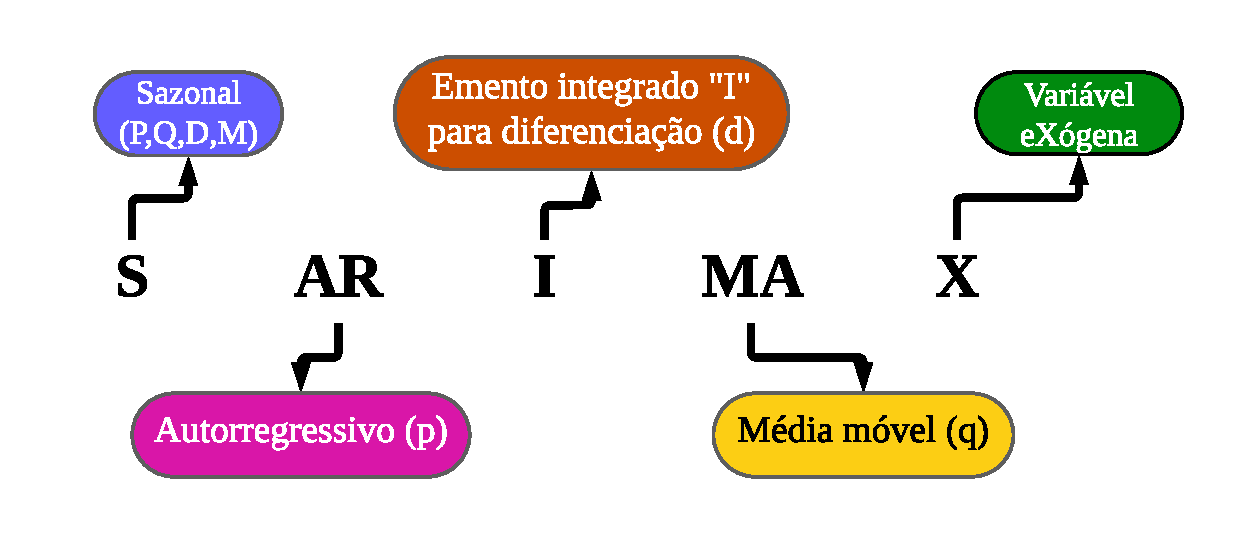
\includegraphics[width=\linewidth]{Modelos/Figuras/sarimax_map.pdf}
 	
 \end{figure}
 
  \subsection{Autocorrela\c c\~ao e Autocorrela\c c\~ao Parcial}
 
As Figuras contendo os gráficos da Função de Autocorrelação (ACF) e da Função de Autocorrelação Parcial (PACF) são ferramentas essenciais na análise de séries temporais, especialmente ao trabalhar com modelos ARIMA. Elas são expressas da seguinte forma:

\begin{eqnarray}
	 R_k &=& \frac{\gamma_k}{\gamma_0} \\ 
	 \phi_{kk} &=& \frac{\gamma_{kk} - \sum_{j=1}^{k-1} \phi_{k-1,j} \gamma_{k-j,k}}{\gamma_{0,k}}
\end{eqnarray}

\noindent onde $ R_k $ é a autocorrelação de ordem $ k $, $ \gamma_k $ é a função de autocovariância de ordem $ k $, $ \phi_{kk} $ é a autocorrelação parcial de ordem $ k $, $ \gamma_{kk} $ é a autocovariância de ordem $ k $, $ \gamma_{0,k} $ é a variância amostral no tempo $ k $, e $ \phi_{k-1,j} $ é a autocorrelação parcial de ordem $ j $ na equação da PACF.
 
 O ACF é uma medida estatística utilizada para identificar a presença de correlação serial em uma série temporal. Ele calcula a autocorrelação entre os valores da série em diferentes defasagens, ou seja, a correlação entre os valores atuais e os valores passados da série. O ACF é útil para analisar a dependência temporal dos dados e identificar padrões de sazonalidade, tendência ou outros efeitos temporais. Por meio do ACF, é possível avaliar se a série exibe autocorrelação significativa em defasagens específicas, o que pode indicar a presença de não estacionariedade ou estrutura temporal que precisa ser considerada na análise ou modelagem da série temporal.
 
 Enquanto o ACF mede a correlação total em um determinado lag, o PACF mede a correlação apenas entre a observação atual e uma observação em um lag específico, controlando os efeitos das observações intermediárias. O gráfico PACF é especialmente útil para identificar a ordem do componente autorregressivo (AR) no modelo ARIMA. Ele ajuda a identificar os lags que têm uma influência direta na observação atual, sem a interferência de outros lags. Ao usar esses gráficos em conjunto, os analistas de séries temporais podem identificar a ordem adequada do modelo ARIMA. 
 
 A ordem do ARIMA é denotada como ($p, d, q$), onde p é a ordem do componente AR, d é a ordem de diferenciação, que representa o número de vezes que a série temporal é diferenciada para torná-la estacionária, e q é a ordem do componente de MA. Os pontos nos gráficos ACF e PACF que ultrapassam as bandas de confiança indicam lags significativos. Analisando esses gráficos, pode fazer escolhas sobre os valores de $p$, $d$, e $q$ ao ajustar um modelo ARIMA à série temporal em questão. 
 
 Na Figura \ref{fig:acfa}, pode-se observar a diferença entre ACF exibida na Figura \ref{fig:acfa} e PACF exibida na Figura \ref{fig:pacf}. A autocorrelação é uma medida da correlação entre os valores da série temporal em diferentes defasagens, levando em consideração tanto a correlação direta quanto a correlação indireta. Por outro lado, a autocorrelação parcial mede apenas a correlação direta entre os valores, desconsiderando a influência das defasagens intermediárias. Essas análises são úteis para identificar padrões e relações de dependência entre os valores da série temporal, fornecendo informações importantes para a modelagem e previsão desses dados. O intervalo de confiança padrão de $95\%$ é representado pela faixa azul nas Figuras \ref{fig:acfa} e \ref{fig:pacf}. As observações que estão fora desse intervalo são consideradas estatisticamente correlacionadas, indicando a presença de padrões ou estrutura na série temporal.
 

 
 \begin{figure}[!htb]
 	\centering
 	\caption{Autocorrelação.}\label{fig:acfa}	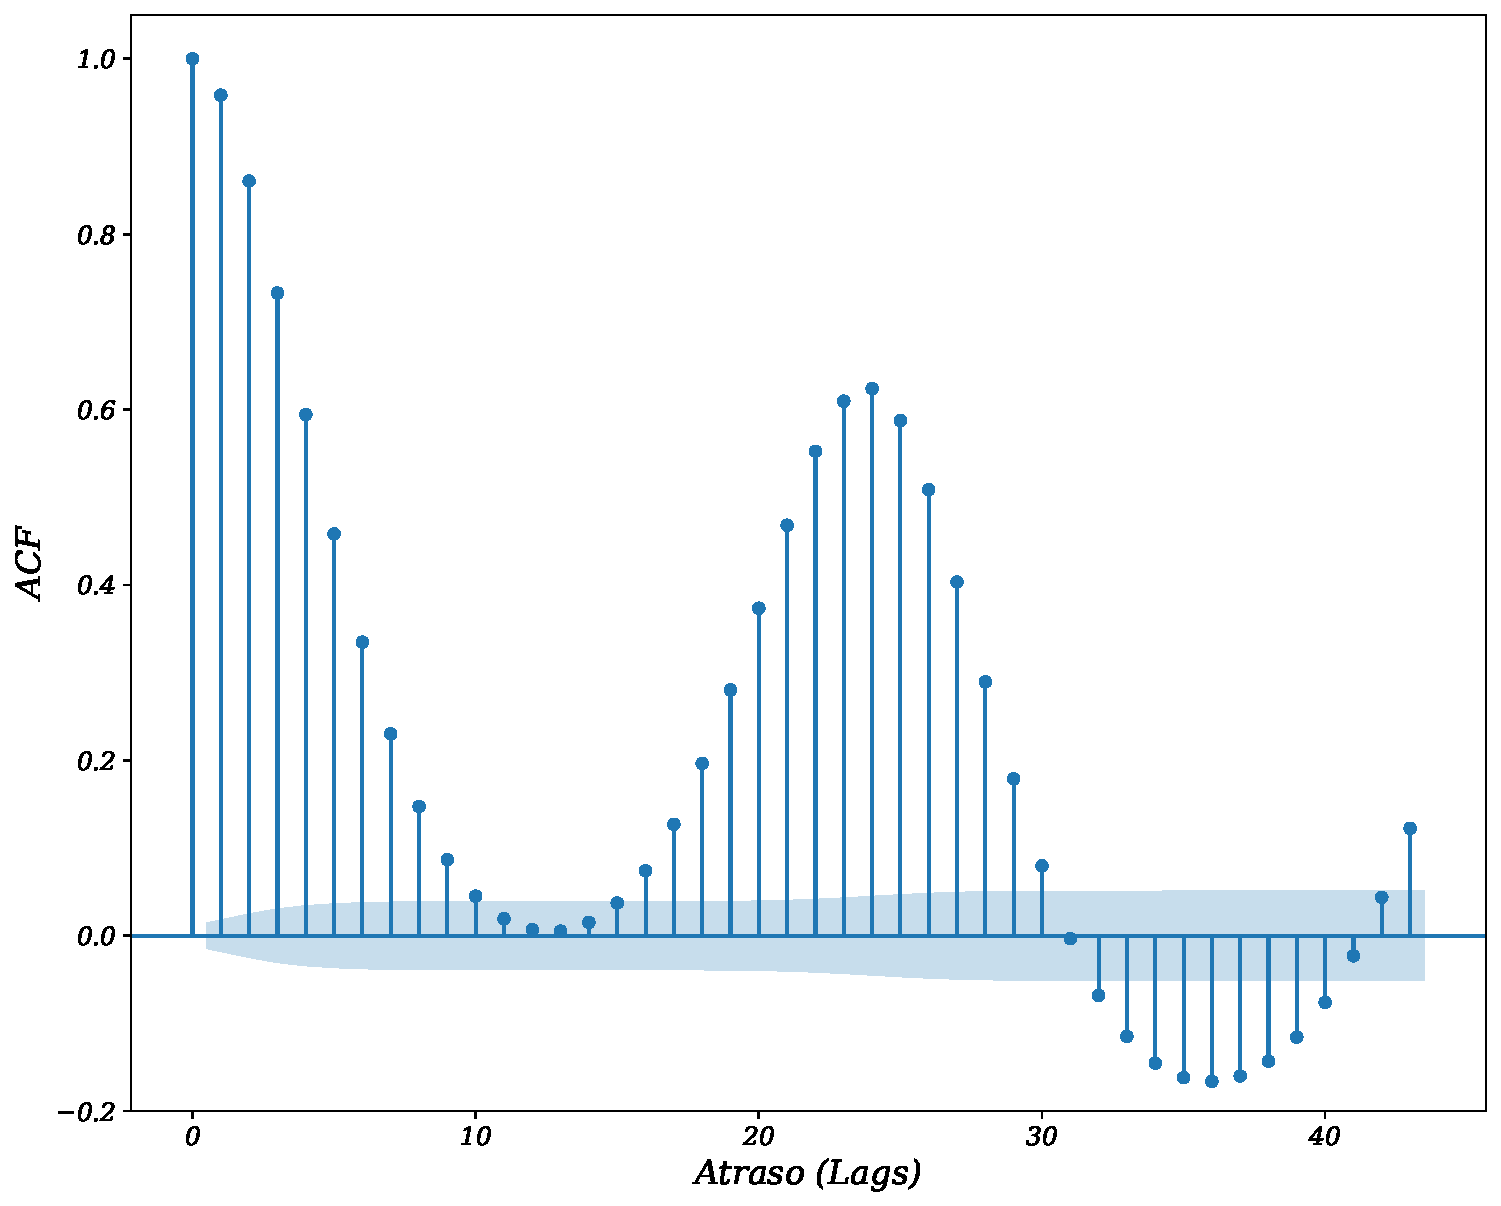
\includegraphics[width=0.6\linewidth]{Resultados/Figuras/acf} 
 \end{figure}
 
 \begin{figure}[!htb]
 	\centering
 	\caption{Autocorrelação parcial.}\label{fig:pacf}	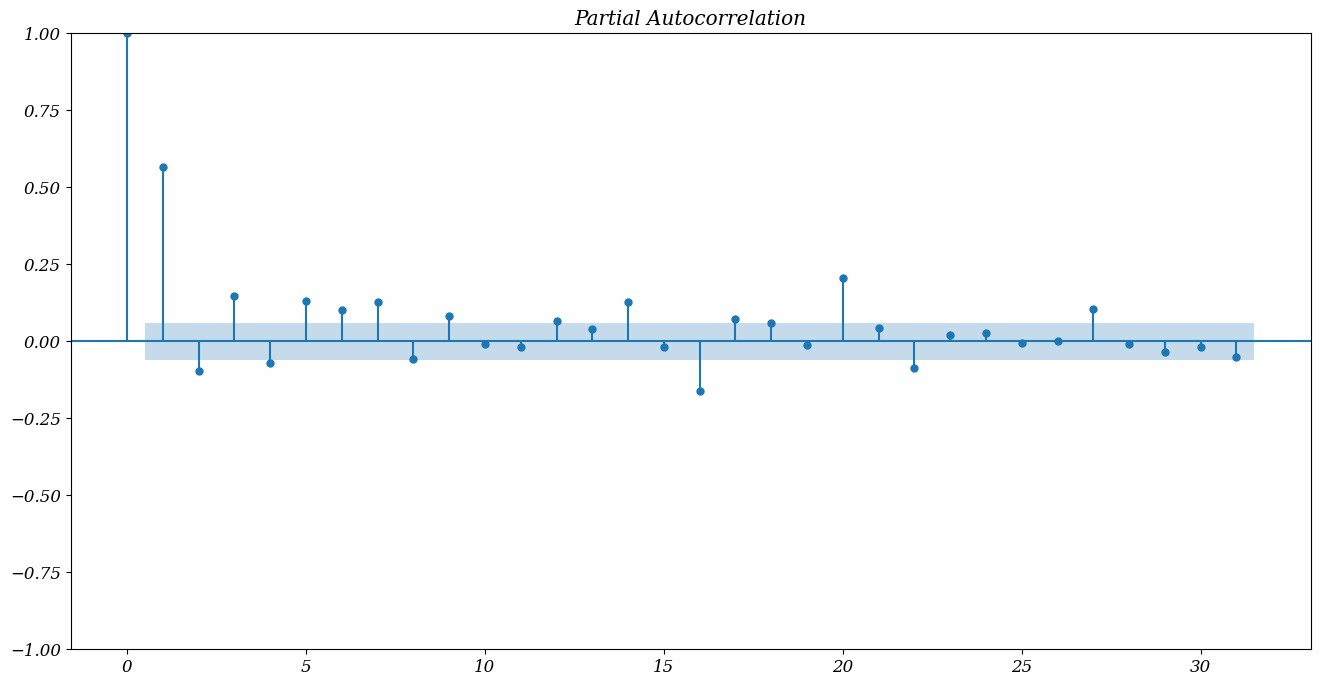
\includegraphics[width=0.6\linewidth]{Resultados/Figuras/pacf}
 \end{figure}
 
 \subsection{Modelos de Aprendizado de M\'aquina}\label{subsec:reg}
 
 Os modelos de aprendizado de máquina para séries temporais têm sido amplamente reconhecidos e utilizados na literatura atual, especialmente por não serem baseados em métodos de gradiente. Esses modelos são valorizados por sua capacidade de capturar relações complexas e não lineares nos dados, permitindo previsões eficientes. Sua popularidade reflete o reconhecimento da eficácia desses modelos em abordar uma ampla gama de problemas de previsão de séries temporais em diferentes áreas de estudo \cite{al2021machine, sen2022machine, kheiri2023sentimentgpt}. A seguir são mencionados alguns dos modelos de aprendizado de máquina utilizados e analisados neste estudo.
 
  \subsubsection{Prophet}
 
 O Prophet é um modelo de previsão de séries temporais desenvolvido pelo Facebook. Foi projetado para simplificar a previsão de séries temporais que apresentam padrões sazonais, tendências e feriados. O Prophet é útil para usuários que desejam realizar previsões sem requerer um profundo conhecimento em estatística ou aprendizado de máquina \cite{en16031371}. O modelo se baseia em uma abordagem aditiva que desagrega a série temporal em vários componentes individuais, como tendência de longo prazo, sazonalidade semanal e anual, e efeitos de feriados. Esses componentes são combinados para formar uma previsão geral.  A equação básica do modelo Prophet pode ser representada da seguinte forma:
 
 \begin{eqnarray}
 	p(t) &=& g(t) + s(t) + h(t) + \varepsilon_t 
 \end{eqnarray}
 
 \noindent onde $ p(t) $ é o valor da série temporal no tempo $ t $, que se deseja prever, $ g(t) $ representa a tendência de longo prazo da série, $ s(t) $ representa os componentes sazonais, que podem incluir padrões semanais e anuais, $ h(t) $ é a representação dos efeitos de feriados ou eventos especiais.
  
 O modelo Prophet ajusta esses componentes aos dados históricos de séries temporais para criar uma previsão futura. Ele utiliza um procedimento de ajuste automático para estimar os parâmetros desses componentes com base nos dados fornecidos. A abordagem aditiva do Prophet permite que os padrões sazonais, tendências e feriados sejam capturados separadamente e, em seguida, somados para gerar uma previsão global \cite{2-s2.0-85092514286}.
 
 
 \subsubsection{Regress\~ao Linear}
 
A regressão linear é classificada como um modelo de aprendizado de máquina supervisionado. Essa classificação é baseada em sua definição, que pode ser formulada da seguinte maneira:
 
 \begin{equation}
 	y = \beta_0 + \beta_1 x_1 + \cdots + \beta_p x_p + \varepsilon \label{eq:lr}
 \end{equation}
 
 \noindent onde há $p$ variáveis explicativas, denotadas por $x$. Existe uma variável alvo, denotada por $y$. O valor de $y$ é calculado como uma constante $\beta_0$, somada aos valores das variáveis $x$ multiplicados por seus coeficientes $\beta_1$ a $\beta_p$.
 
 
 Para utilizar a regressão linear \cite{korstanje2021}, é necessário estimar os coeficientes beta com base em um conjunto de dados de treinamento. Esses coeficientes podem ser estimados por meio de,
 
 \begin{eqnarray}
 	\hat{\beta}&=&\left(X^T X\right)^{-1} X^T y\label{eq:ols}
 \end{eqnarray}
 
 \noindent onde, $\hat{\beta}$ é um vetor de coeficientes estimados que minimiza a soma dos quadrados dos resíduos no método de mínimos quadrados ordinários  \textit{Ordinary Least Squares method} (OLS). Cada $\hat{\beta}_i$ representa o coeficiente estimado para a variável independente $X_i$;
 $X$ é a matriz de dados independentes, onde cada coluna representa uma variável independente diferente e cada linha representa uma observação separada;
 resultando no vetor de coeficientes.
 
 
 \subsubsection{\'Arvore de Decis\~ao}
 
 Uma árvore de decisão é um dos modelos de aprendizado de máquina frequentemente utilizados para resolver problemas de regressão e classificação. Como o nome sugere, o algoritmo utiliza um modelo de decisões semelhante a uma árvore para prever o valor de destino (regressão) ou determinar a classe de destino (classificação) \cite{SHI2023110022}. É importante se familiarizar com as terminologias básicas associadas a uma árvore de decisão \cite{SINGHKUSHWAH20223571}.
 
 Na Figura \ref{fig:decison} tem-se o nó raiz que é o nó mais alto da árvore que representa todos os pontos de dados. A divisão refere-se à criação de um nó em dois ou mais sub-nós.
 O nó de decisão são os nós que são divididos em sub-nós, ou seja, esse nó que é dividido é chamado de nó de decisão. O nó folha/terminal são os nós que não se dividem. Esses nós estão geralmente no final da árvore. O ramo/subárvore é uma subseção de toda a árvore e é chamada de galho ou subárvore. O nó pai e filho é um nó, que é dividido em sub-nós e é chamado de um nó pai de sub-nós, enquanto sub-nós são os filhos do nó pai. Na Figura \ref{fig:decison}, o nó de decisão é o pai dos nós terminais (filhos).
 A poda é a remoção de sub-nós de um nó de decisão. A poda costuma ser feita em árvores de decisão para evitar o \textit{overfitting}  \cite{decision}.
 
 \begin{figure}[H]
 	\centering
 	\caption{Fluxograma da árvore de decisão.}
 	\label{fig:decison}
 	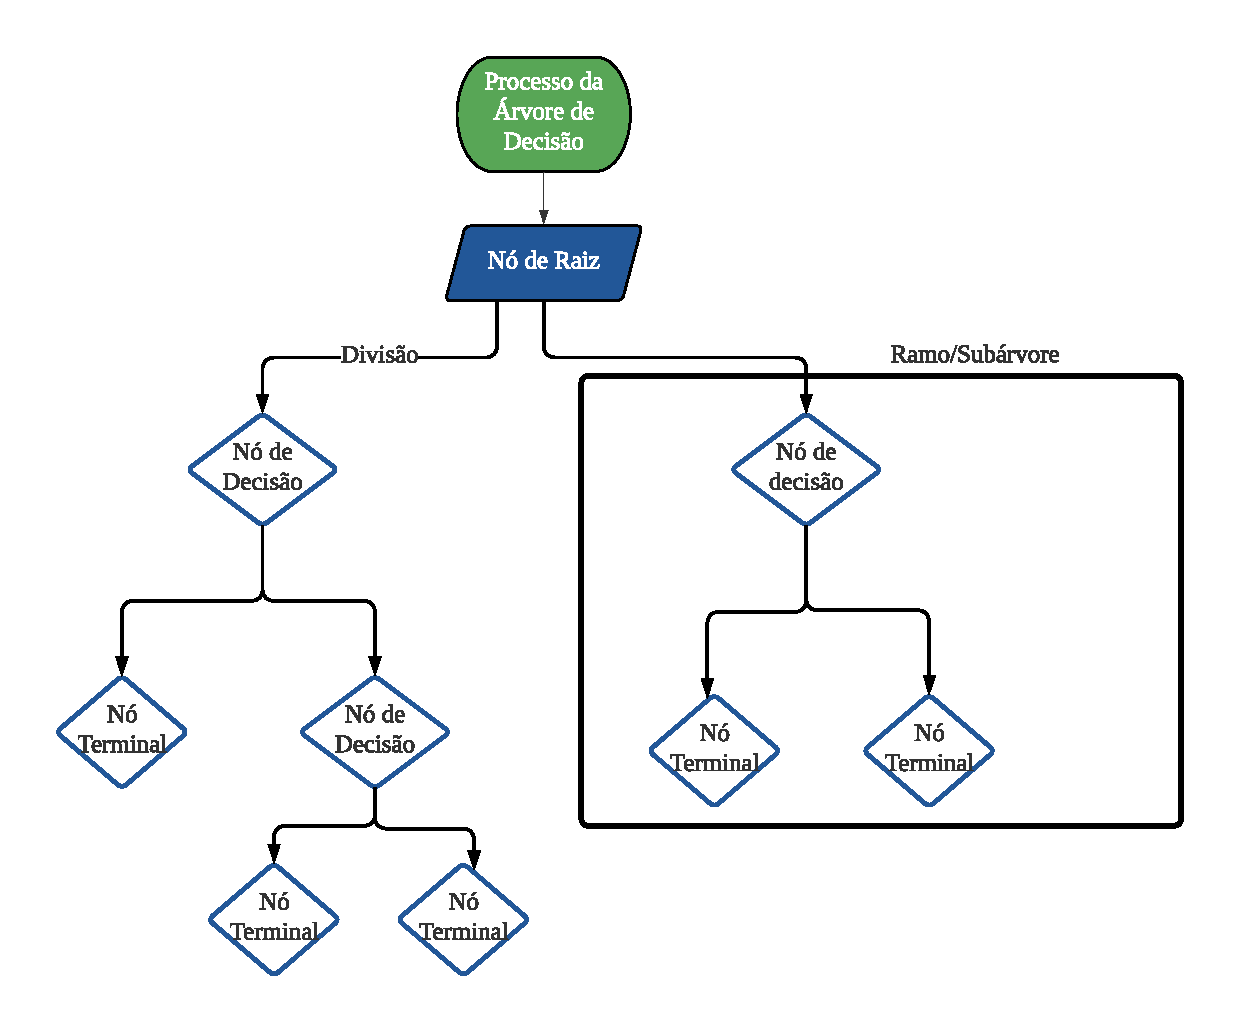
\includegraphics[width=0.7\linewidth]{Modelos/Figuras/decison.pdf}
 	
 \end{figure}
  
 A árvore de decisão pode ser mais robusta que modelo de regressão linear, tendo a capacidade de otimizar os parâmetros para trabalhar com horizontes de tempo mais longos. Vale destacar novamente, que a árvore de decisão representa um conjunto de regras de decisão hierárquicas, organizadas na forma de uma árvore. Cada nó na árvore representa uma decisão ou teste sobre um atributo, e cada ramo representa um possível resultado dessa decisão \cite{GIFFORD2023100296}. Observa-se analisando a Figura \ref{fig:decison} que repetir exatamente a mesma árvore de decisão várias vezes não adiciona valor significativo em comparação com o uso dessa árvore de decisão apenas uma vez. Em modelos de conjunto, é crucial que cada modelo individual apresente pequenas variações em relação aos demais.
 

Cada nó na árvore representa uma decisão ou teste sobre um atributo, e cada ramo representa um possível resultado dessa decisão. Considerando a Figura \ref{fig:decison} como exemplo, a estrutura da árvore pode ser representada matematicamente da seguinte forma:
 
 $$ F(x) = \begin{cases} 
 	f_1(x) & \text{se } x \text{ pertence à região do Nó 1} \\
 	f_2(x) & \text{se } x \text{ pertence à região do Nó 2} \\
 	\vdots \\
 	f_k(x) & \text{se } x \text{ pertence à região do Nó } k 
 \end{cases} $$
 
\noindent onde, $ F(x) $ é a função de previsão do modelo de Árvore de Decisão para a instância $ x $, $ k $ representa o número total de folhas na árvore, $ f_i(x) $ é a previsão associada à $ i $-ésima folha, determinada pela sequência de testes nos nós da árvore.

Cada teste nos nós da árvore compara um atributo específico de $ x $ com um valor de corte, decidindo qual ramo da árvore seguir com base no resultado. Este processo continua até que $ x $ chegue a uma folha, e a previsão associada a essa folha é atribuída a $ F(x) $. Vale destacar que a robustez da árvore de decisão permite otimizar os parâmetros para lidar com horizontes de tempo mais longos, sendo uma alternativa mais flexível em comparação com modelos de regressão linear.
 
 
  
 \subsubsection{Floresta Aleat\'oria} \label{subsubsec:rf}
 
Dois modelos de previsão amplamente reconhecidos para criar conjuntos são \textit{bagging} e \textit{boosting}. A floresta aleatória RF utiliza o ensacamento para criar um conjunto de árvores de decisão, onde cada árvore é construída com uma amostra aleatória do conjunto de dados original. Isso assegura que as árvores sejam distintas e diversificadas, contribuindo para a robustez e eficácia do modelo \cite{SEMAN2023109269}.
 
 Cada árvore da RF é construída por meio de um algoritmo de aprendizado individual que divide o conjunto de variáveis de entrada em subconjuntos, com base em um teste de valor de atributo, como o coeficiente de Gini. Ao contrário das árvores de decisão clássicas, as árvores do modelo RF são construídas sem poda e selecionam aleatoriamente um subconjunto de variáveis de entrada em cada nó. Atualmente, o número de variáveis utilizadas para dividir um nó em uma RF, denotado por $m$, corresponde à raiz quadrada do número total de variáveis de entrada. 
 
 Essa abordagem ajuda a aumentar a diversidade das árvores e aprimorar o desempenho do modelo \cite{Pelletier2016156}. Na Figura \ref{fig:rf}, um fluxograma do modelo RF ilustra como as árvores funcionam.
 Na construção da próxima árvore, os dois processos anteriores se repetirão, levando à criação de uma nova árvore. Provavelmente, essa árvore será diferente da primeira, pois tanto na seleção das amostras quanto na seleção das variáveis, o processo ocorre de maneira aleatória.
  
 \begin{figure}[!htb]
 	\centering
 	\caption{Fluxograma da floresta aleatória.}
 	\label{fig:rf}
 	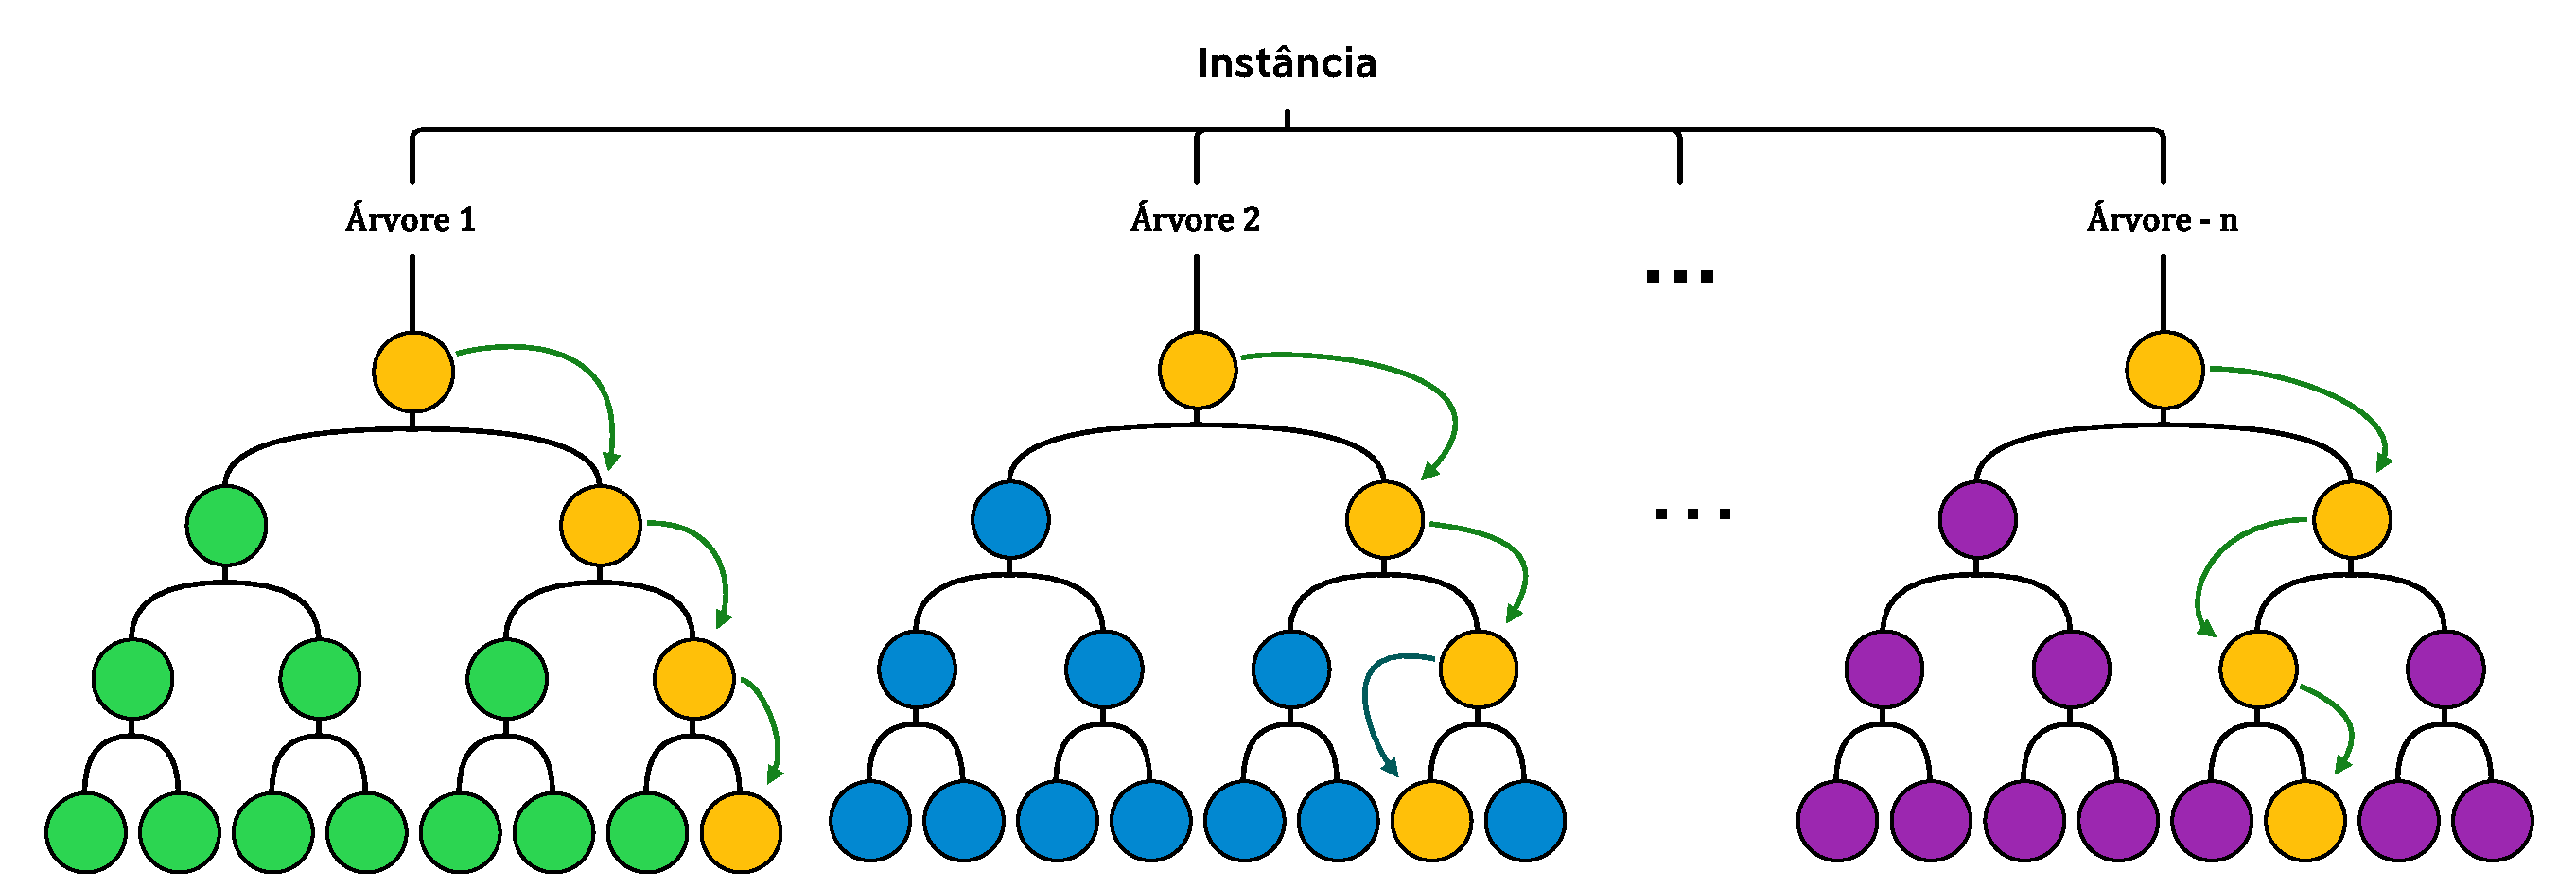
\includegraphics[width=\linewidth]{Modelos/Figuras/RF.pdf}
 \end{figure}
 
A opção pelo modelo RF em detrimento do modelo árvore de decisão é motivada por várias vantagens em termos de desempenho, robustez e generalização. Ele se destaca por apresentar uma redução significativa do \textit{overfitting}, garantindo uma abordagem mais estável e resistente a variações nos dados. Além disso, a capacidade do RF de lidar com um grande número de características e determinar a importância relativa de cada uma contribui para uma melhor compreensão e interpretação do conjunto de dados. Essas características fazem do RF uma escolha valiosa em contextos onde é crucial alcançar resultados mais precisos e gerais.

Seja $ F(x) $ a função de previsão da Floresta Aleatória para a instância $ x $, e $ T_i(x) $ a previsão da $ i $--ésima árvore na floresta. Então, a previsão final da Floresta Aleatória é dada por:

\begin{eqnarray}
	F(x) &=& \frac{1}{N} \sum_{i=1}^{N} T_i(x) 
\end{eqnarray}

\noindent onde, $ N $ é o número total de árvores na floresta. Cada árvore $ T_i(x) $ é construída com uma amostra aleatória do conjunto de dados original, garantindo a diversidade e robustez do modelo. A previsão de cada árvore é combinada através da média, proporcionando uma abordagem de conjunto para melhorar a precisão e generalização do modelo.
 
 \subsubsection{\textit{Gradient Boosting}}\label{subsubsec:lgbxgb}
 
 O \textit{Gradient Boosting} é um modelo que combina vários modelos de árvore de decisão para realizar previsões. Cada uma dessas árvores de decisão é única, pois a diversidade é um elemento importante nesse processo. A diversidade é alcançada através de um processo chamado \textit{boosting}, que é uma abordagem iterativa, que adiciona modelos fracos ao conjunto de forma inteligente, dando peso maior aos pontos de dados que ainda não foram previstos de forma adequada \cite{BUEECHI2023109596}. 
 
A Figura \ref{fig:xgboos} apresenta uma visão esquemática do modelo XGBoost. À medida que novos modelos fracos são adicionados, todos os modelos fracos intermediários são mantidos. O modelo final é uma combinação de todos esses modelos fracos, resultando em um ensemble que oferece uma melhor capacidade de previsão do que um único modelo.

\begin{figure}[!htb]
	\centering
	\caption{Fluxograma do XGBoost}
	\label{fig:xgboos}
	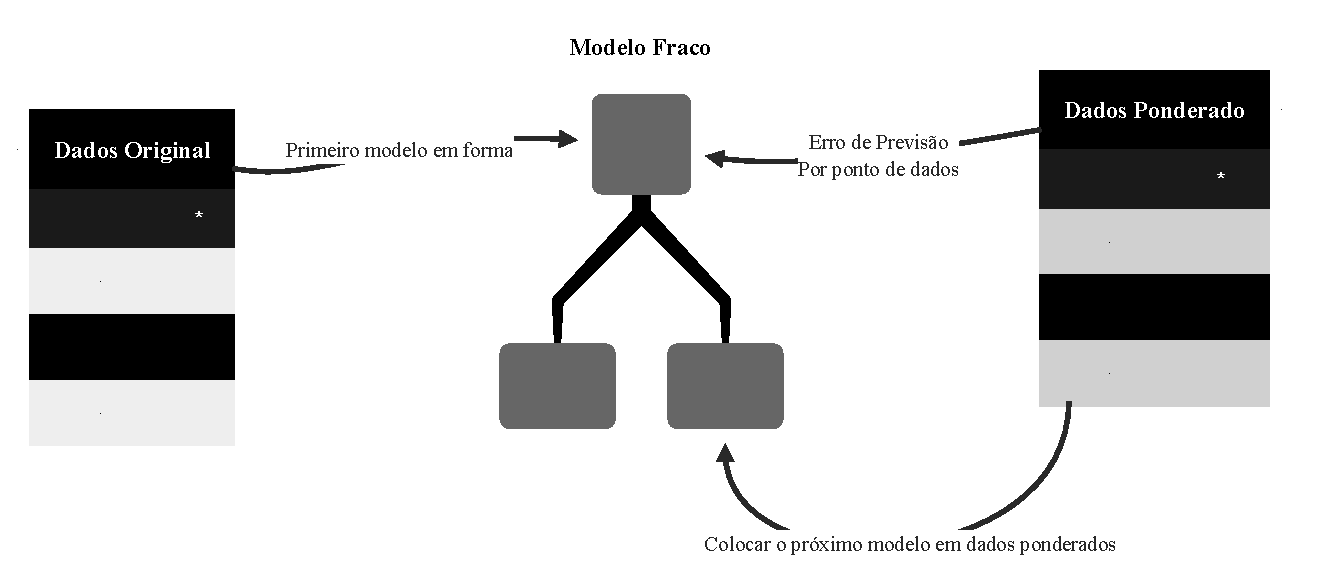
\includegraphics[width=\linewidth]{Modelos/Figuras/xgboos.pdf}
\end{figure}
 

 \begin{eqnarray}
 	 F(x) &=& \sum_{i=1}^{T} f_t(x) \label{eq:xgboost}
 \end{eqnarray}

 
\noindent na equação \eqref{eq:xgboost}, $F(x)$ é a função de previsão final do modelo,  $T$ é o número total de árvores de decisão no modelo, $f_t(x)$  representa a saída da árvore de decisão $ t $ para a instância $ x $.
 
 O processo de treinamento do XGBoost envolve a minimização de uma função de perda regularizada, que incorpora termos para penalizar a complexidade do modelo e reduzir o \textit{overfitting}. Isso é feito através de um processo iterativo, onde novas árvores são adicionadas ao modelo, e a cada iteração, a função de perda é otimizada. A diversidade entre as árvores é garantida pela atribuição de pesos diferentes a cada uma, considerando seus erros residuais.
 

\begin{eqnarray}
	 \text{Objetivo} &=& \sum_{i=1}^{n} L(y_i, \hat{y}_i) + \sum_{k=1}^{T} \Omega(f_k) \label{eq:xgboost1}
\end{eqnarray}

 
 \noindent na equação \eqref{eq:xgboost1}, $ L(y_i, \hat{y}_i) $ é a função de perda que mede a discrepância entre a previsão $ \hat{y}_i $ e o rótulo verdadeiro $ y_i $, $ \Omega(f_k) $ é um termo de regularização que penaliza a complexidade da $ k $--ésima árvore, a função objetivo é uma combinação da função de perda e termos de regularização.
 
 Esse processo de otimização é efetuado através de técnicas como \textit{Gradient Boosting}, que ajusta os modelos fracos sequencialmente para melhorar a precisão global do modelo.
 

 
 \subsubsection{\textit{LightGBM}}
 
 Uma alternativa proposta pelo XGBoost é a segmentação baseada em histograma. Nesse caso, em vez de iterar por todas as partições possíveis, o modelo constrói um histograma para cada variável e utiliza-os para encontrar a melhor divisão geral entre as variáveis. O LightGBM, desenvolvido pela Microsoft, adota uma abordagem mais eficiente para a definição das divisões. Essa abordagem é conhecida como amostragem \textit{Gradient-Based One-Side Sample} (GOSS). O GOSS calcula o gradiente para cada ponto de dados e utiliza-o para filtrar os pontos de dados com gradientes baixos \cite{SUN2020101084}. 
 
 O LightGBM também utiliza uma abordagem chamada \textit{Exclusive Feature Bundling} (EFB), que acelera a seleção de variáveis correlacionadas. 
 Outra diferença é que o modelo LightGBM é adequado para o crescimento de folhas, enquanto o XGBoost cultiva as árvores em níveis. Essa diferença pode ser visualizada na Figura \ref{fig:xgboost} \cite{YE2023407}. Essa diferença teoricamente favorece o LightGBM em termos de precisão, mas também apresenta um maior risco de sobre-ajuste quando há poucos dados disponíveis. 
 
 Na Figura \ref{fig:xgboost}, é possível visualizar como cada modelo é ajustado durante o processo de crescimento de árvore em folhas e em níveis. Essa representação gráfica oferece uma compreensão visual das diferenças entre os modelos. A Figura \ref{fig:xgboost}, apresenta um diagrama que ilustra o crescimento de uma árvore em termos de níveis, modelo XGBoost, e crescimento de uma árvore em termos de folhas, modelo LightGBM.
 
 \begin{figure}[!htb]
 	\centering
 	\caption{Comparação do crescimento em folha com o crescimento em nível}
 	\label{fig:xgboost}
 	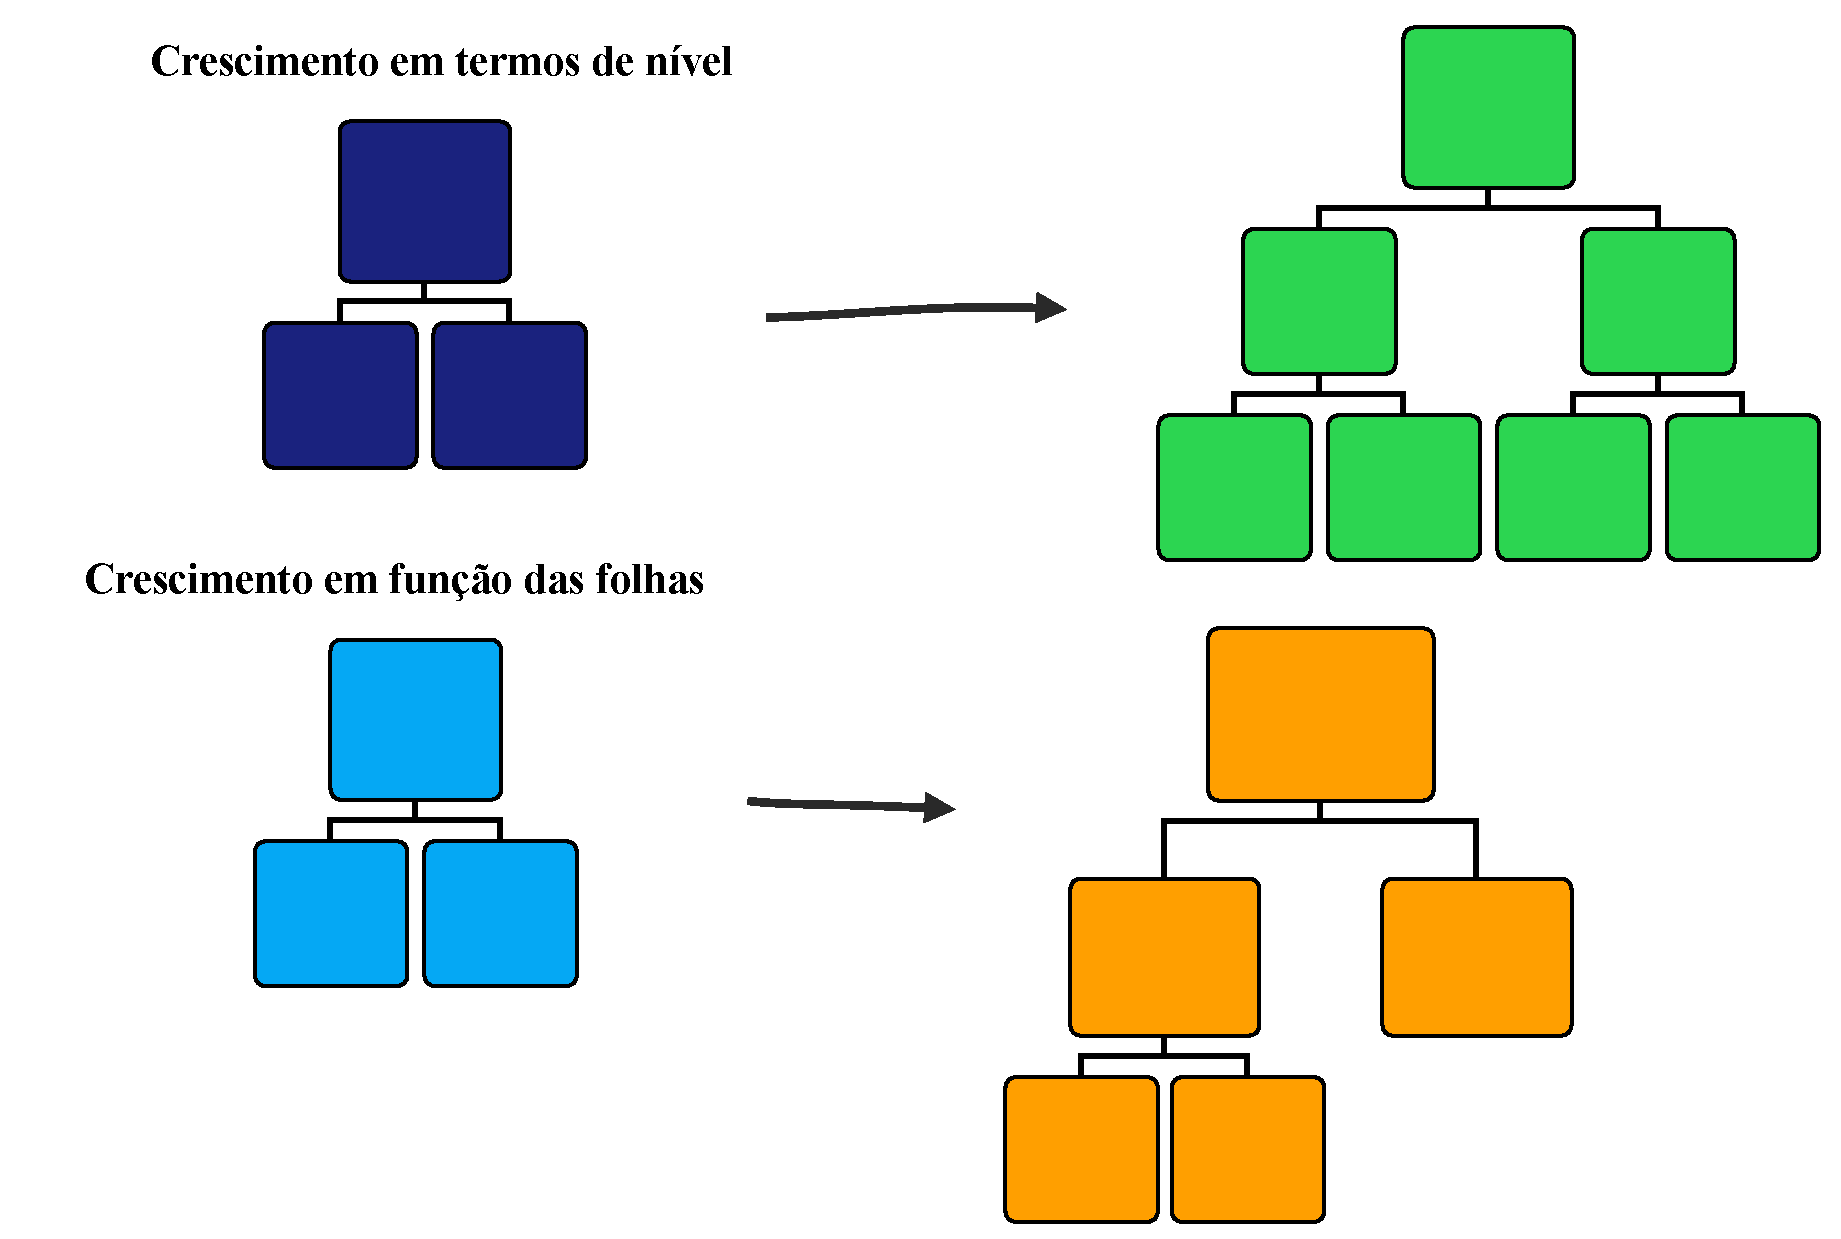
\includegraphics[width=0.7\linewidth]{Modelos/Figuras/xgboost.pdf}
 \end{figure}
 
 
 No crescimento de árvore em folhas, no modelo LightGBM, novas folhas são adicionadas à árvore de forma iterativa, visando maximizar a redução do erro de treinamento. Isso significa que as árvores são expandidas adicionando folhas, uma a uma, até que o critério de parada seja alcançado.  No crescimento em níveis, no modelo XGBoost, as árvores são expandidas em profundidade de forma simultânea em todos os níveis. Ou seja, em cada nível, todas as folhas são expandidas ao mesmo tempo, resultando em um crescimento mais uniforme da árvore. Essa distinção no modo de crescimento das árvores pode afetar o comportamento e o desempenho do modelo. 
  
 \noindent\textbf{XGBoost:}
 
 A função de previsão do modelo XGBoost para a instância $x$ é representada por $F_{\text{XGBoost}}(x)$. Esta função é obtida através do crescimento de árvores em níveis, onde cada árvore é construída simultaneamente em profundidade em todos os níveis. Assim, a previsão final é dada por:
 
 \begin{eqnarray}
 F_{\text{XGBoost}}(x) &=& \sum_{i=1}^{N} T_i(x)
 \end{eqnarray}
 
 \noindent onde $N$ é o número total de árvores na floresta, e $T_i(x)$ representa a previsão da $i$-ésima árvore.
 
\noindent\textbf{LightGBM:}
 
 A função de previsão do modelo LightGBM para a instância $x$ é representada por $F_{\text{LightGBM}}(x)$. A abordagem do LightGBM inclui a amostragem \textit{Gradient-Based One-Side Sample} (GOSS) para filtrar pontos de dados com gradientes baixos, e o \textit{Exclusive Feature Bundling} (EFB) para acelerar a seleção de variáveis correlacionadas. A previsão final é dada por:
 

\begin{eqnarray}
	 F_{\text{LightGBM}}(x) &=& \sum_{i=1}^{N} T_i(x)
\end{eqnarray}

 
 \noindent onde, $N$ é o número total de árvores na floresta, e $T_i(x)$ representa a previsão da $i$-ésima árvore. No LightGBM, as árvores são cultivadas adicionando folhas iterativamente para maximizar a redução do erro de treinamento, resultando em um crescimento em folhas. Isso contrasta com o XGBoost, que expande as árvores em profundidade simultaneamente em todos os níveis, resultando em um crescimento mais uniforme da árvore.
  
  
 \subsection{Redes Neurais Artificiais}
 
 Uma rede neural é um modelo de processamento de informações inspirado pelo funcionamento do cérebro humano. Consiste em um conjunto interconectado de unidades de processamento, conhecidas como neurônios artificiais, que trabalham em conjunto para realizar tarefas de aprendizado a partir de dados \cite{XIANG2018874}. Assim como os neurônios no cérebro estão interligados por sinapses, os neurônios artificiais são conectados por conexões ponderadas. Essas conexões permitem que a rede neural analise padrões complexos nos dados, reconhecendo relações e características importantes para executar tarefas como classificação, previsão, reconhecimento de padrões \cite{BABU201427}. Conforme a rede é exposta a exemplos e informações, ela ajusta suas conexões para melhorar seu desempenho, tornando-a capaz de generalizar e lidar com novos dados \cite{RAO2020107851}.

\subsubsection{MLP}
 
Uma Rede Neural MLP é um tipo de arquitetura de rede neural artificial composta por várias camadas de neurônios (ou unidades) organizados em uma estrutura de múltiplas camadas. Cada neurônio em uma camada está conectado a todos os neurônios da camada seguinte, sem formar ciclos (rede \textit{feedforward}). Essa arquitetura é projetada para realizar tarefas de aprendizado supervisionado, como classificação e regressão \cite{QIN2023543}.

 A topologia da MLP funciona como uma rede \textit{feedforward}, rede progressiva, a saída de um neurônio se conecta com outro neurônio da próxima camada, no sentido esquerda/direita, formada por um conjunto de neurônios denominados nós, como  na Figura \ref{fig:ann}. A rede possui uma camada de entrada, sem função de ativação, uma ou mais camadas ocultas e uma camada de saída. A complexidade da rede neural MLP se dá pela quantidade de camadas ocultas que houver e a quantidade de neurônios que essas camadas possuírem \cite{Grubler2018}.
 
 \begin{figure}[!htb]
 	\centering
 	\caption{Modelo de uma rede neural artificial MLP.}
 	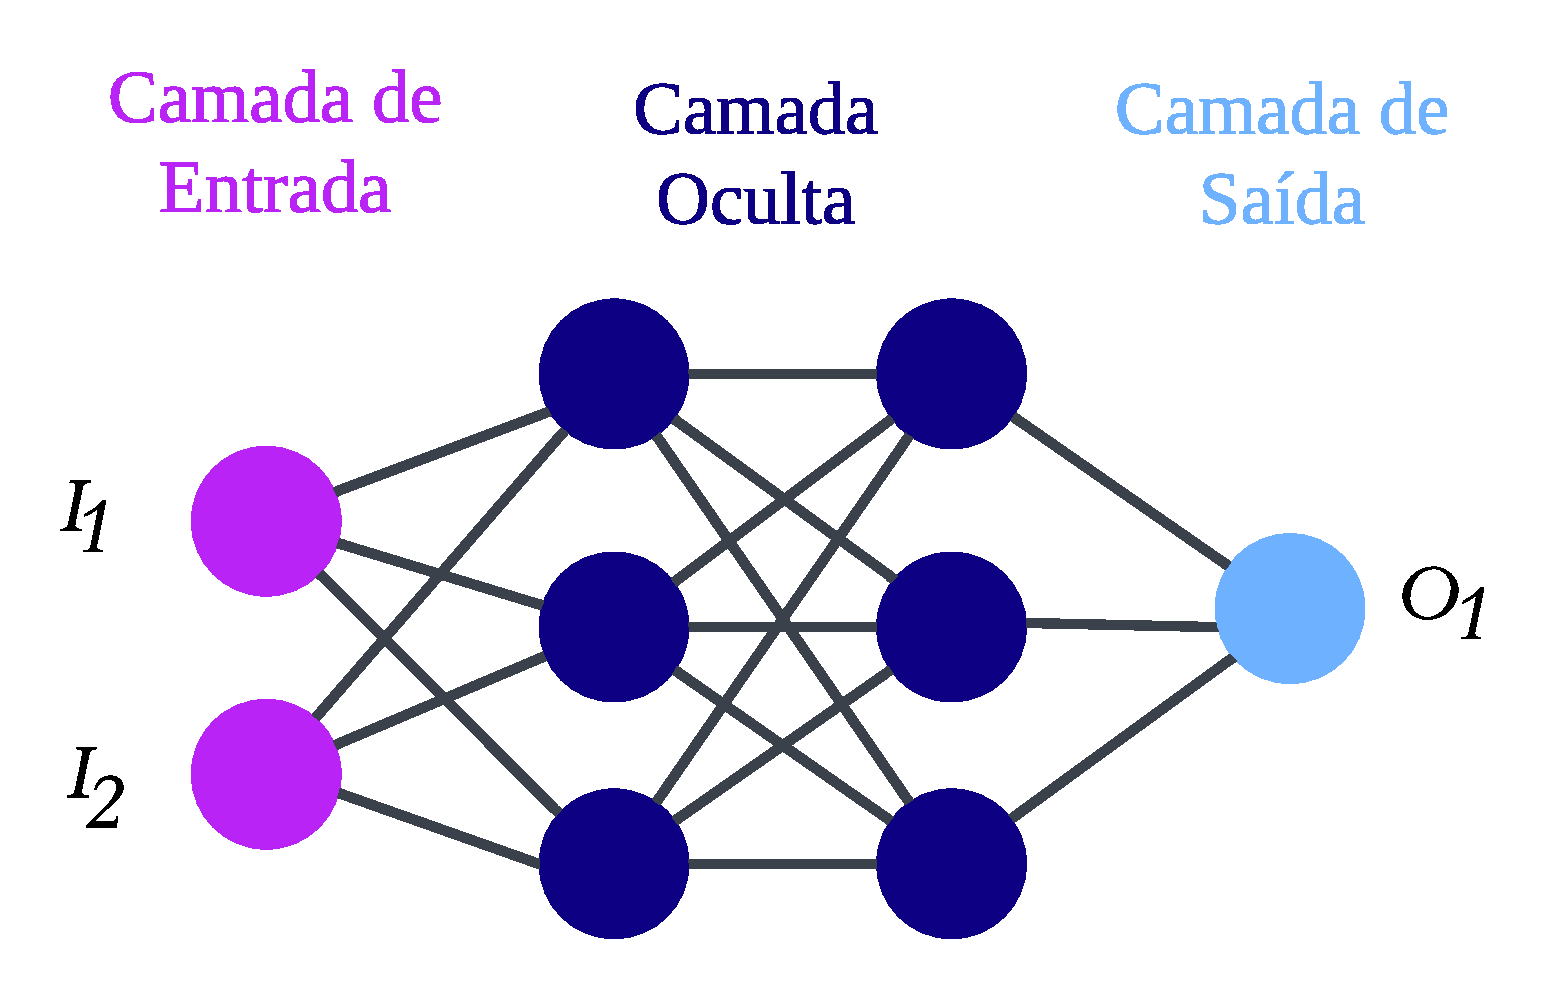
\includegraphics[width=0.5\linewidth]{Modelos/Figuras/ann.pdf}
 	
 	\label{fig:ann}
  \end{figure}
 
 \begin{equation}
 	\begin{aligned}
 		& I=\left[I_1, I_2\right]=\text { Vetor de Entrada } \\
 		& O=\left[O_1\right]=\text { Vetor de Saída }
 	\end{aligned} \nonumber
 \end{equation}
 
 O modelo de rede neural artificial MLP é dado por,
 
 \begin{eqnarray}
 	v_j=\sum_{i=0}^m w_i y_i+b\label{eq:ann}
 \end{eqnarray}
 
 \noindent o funcionamento geral de uma rede MLP está representada na Figura \ref{fig:ann}. Cada neurônio recebe todos os valores das entradas, representadas pelo símbolo $y$, que são multiplicadas pelos pesos sinápticos simbolizados pelo $w$ e somadas entre si junto com uma constante chamada de polarização ou bias, representada pelo símbolo $b$.
 
  \subsubsection{Rede Neural Recorrente}
  
 Uma Rede Neural Recorrente RNN é um tipo de arquitetura de rede neural que pode ser utilizada para usar dados sequenciais ou temporais \cite{NASIRI2023110867}. Ao contrário das redes neurais convencionais, onde as entradas e saídas são tratadas como dados independentes, as RNNs levam em consideração a ordem e a relação entre os elementos em uma sequência, tornando-as ideais para lidar com dados como séries temporais.
 
 A característica principal das RNNs é que elas contêm laços em sua estrutura, permitindo que informações anteriores influenciem o processamento de informações subsequentes. Isso significa que a saída em um determinado passo de tempo não depende apenas da entrada atual, mas também das entradas anteriores na sequência.
  
 \begin{eqnarray}
 	h_t &=& f(W_{hh} \cdot h_{t-1} + W_{xh} \cdot x_t + b_h)\label{eq:rnn}
 \end{eqnarray}
 
 \noindent onde $ h_t $ é o estado oculto (ou saída) no tempo $ t $, $ h_{t-1} $ é o estado oculto anterior no tempo $ t-1 $, $ x_t $ é a entrada no tempo $ t $, $ W_{hh} $ é a matriz de pesos que controla a influência do estado oculto anterior, $ W_{xh} $ é a matriz de pesos que controla a influência da entrada, $ b_h $ é o vetor de viés, $ f $ é uma função de ativação, frequentemente a função tangente hiperbólica ($\operatorname{tanh}$) ou a função sigmoide \cite{lstm}.
 
 A equação representa a propagação do estado oculto ao longo do tempo em uma RNN. A cada novo passo de tempo, a RNN considera a entrada atual $ x_t $ e o estado oculto anterior $ h_{t-1} $, calculando o novo estado oculto $ h_t $ usando as matrizes de pesos e a função de ativação. 
 
  No entanto, as RNNs tradicionais podem enfrentar dificuldades em capturar dependências de longo prazo, devido ao problema de dissipação do gradiente. Para entender isso, surgiram variações avançadas, como LSTM  e GRU, que incorporam mecanismos de aprendizado de esquecimento e controle de informação, permitindo que informações relevantes sejam mantidas por períodos mais longos de tempo \cite{WANG2023116247}, \cite{ZHAO2023114136}.
 
 Como pode ser visto na Figura \ref{fig:rnn1}, a grande diferença da RNN é que há um laço de reações. Enquanto cada entrada de uma rede totalmente conectada é completamente independente, as entradas de uma RNN têm uma relação de realimentação entre si. Isso faz com que ela seja capaz de capturar padrões em dados sequenciais de uma maneira que redes neurais tradicionais talvez não conseguem.
  
 \begin{figure}[!htb]
 	\centering
 	\caption{Fluxograma da RNN.}
 	\label{fig:rnn1}
 	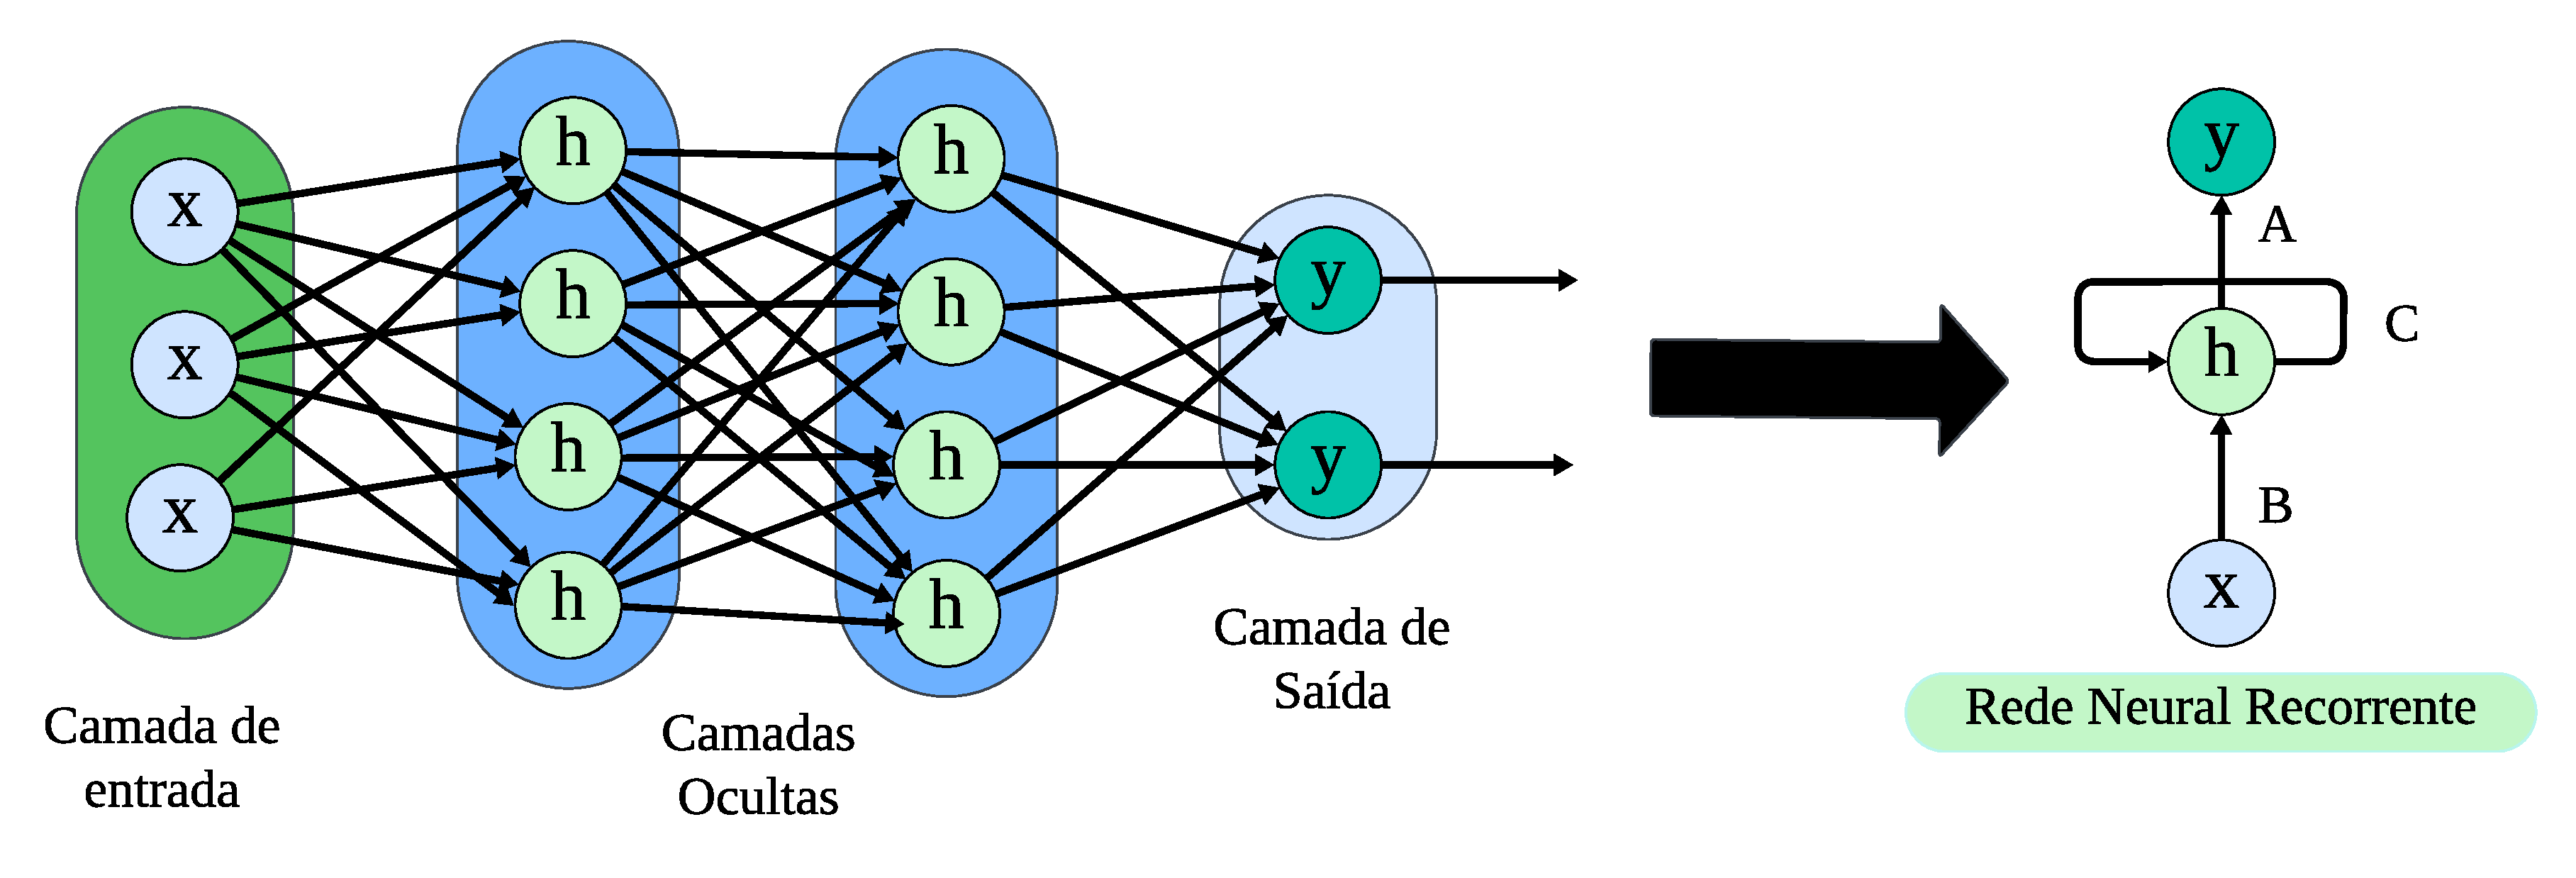
\includegraphics[width=\linewidth]{Modelos/Figuras/rnn1.pdf}
 
 \end{figure}
 
  \subsection{Aprendizado Profundo}

 Aprendizado Profundo ou \textit{Deep Learning} (DL) refere-se a um subcampo do aprendizado de máquina que envolve a construção e o treinamento de modelos de rede neural profunda. O termo profundo se refere ao uso de arquiteturas de modelos que consistem em várias camadas, conhecidas como redes neurais profundas \cite{KOTHONA2023101149}.
 

 
 \subsubsection{LSTM}
 
 As redes neurais LSTMs são uma evolução das RNNs, projetadas para superar desafios na captura de dependências de longo prazo em sequências de dados. Diferentemente das RNNs convencionais, as LSTMs têm a capacidade de manter informações relevantes por longos períodos, tornando-as especialmente eficazes em tarefas que envolvem padrões complexos e dependências temporais distantes \cite{Zhang2021}.
 
 Uma das principais inovações das LSTMs é a introdução de unidades de memória chamadas células, que possuem três componentes principais: uma porta de entrada (\textit{input gate}), uma porta de esquecimento (\textit{forget gate}) e uma porta de saída (\textit{output gate}). Essas portas permitem que as LSTMs controlem o fluxo de informações através da célula, decidindo quais informações devem ser mantidas, esquecidas ou passadas para a saída \cite{Zhang2021}.
  
 \begin{eqnarray}
 	f_t &=& \sigma(W_{xf} \cdot x_t + W_{hf} \cdot h_{t-1} + b_f) \\
 	i_t &=& \sigma(W_{xi} \cdot x_t + W_{hi} \cdot h_{t-1} + b_i) \\
 	\tilde{C}_t &=& \tanh(W_{xc} \cdot x_t + W_{hc} \cdot h_{t-1} + b_c) \\
 	C_t &=& f_t \odot C_{t-1} + i_t \odot \tilde{C}_t \\
 	o_t &=& \sigma(W_{xo} \cdot x_t + W_{ho} \cdot h_{t-1} + b_o) \\
 	h_t &=& o_t \odot \tanh(C_t)
 \end{eqnarray}
 
\noindent onde $x_t$ é a entrada no tempo $t$, $h_{t-1}$ é o estado oculto anterior no tempo $t-1$, $f_t$ é o valor da porta de esquecimento, $i_t$ é o valor da porta de entrada, $\tilde{C}_t$ é o candidato a novo estado de memória, $C_t$ é o novo estado de memória, $o_t$ é o valor da porta de saída, $h_t$ é o novo estado oculto (saída) no tempo $t$, $\sigma$ é a função de ativação sigmoide, $\odot$ representa a multiplicação elemento a elemento.
 
 Essa estrutura permite que as LSTMs controlem o fluxo de informações e aprendam a armazenar ou descartar informações relevantes para diferentes tarefas. As portas de entrada, esquecimento e saída funcionam como mecanismos de controle, permitindo que as LSTMs aprendam a manter informações importantes, esquecer informações desnecessárias e gerar saídas precisas ao longo de sequências temporais.
 
 \subsubsection{GRU}
 
Uma rede neural GRU é um tipo de arquitetura de RNN que foi projetado para trabalhar com o problema de dissipação de gradiente e captura de dependências de longo prazo em sequências de dados. Essa variação das RNNs tradicionais introduz mecanismos para controlar o fluxo de informação por meio das unidades de tempo.
A GRU é uma alternativa vantajosa para a análise de séries temporais, devido à sua habilidade de lidar com sequências de dados de extensões variáveis e de capturar dependências de longo prazo presentes em informações sequenciais. Além disso, a GRU apresenta uma estrutura de simplicidade superior à LSTM, permitindo um processo de treinamento ágil  \cite{mastersthesis53fd58a7}.
 
A estrutura da GRU inclui dois portões principais: o portão de atualização (\textit{update gate}) e o portão de reinicialização (\textit{reset gate}). Esses portões permitem que o GRU decida quais informações serão transmitidas para a próxima etapa de tempo e quais informações serão descartadas, nessas equações 
 
 \eqref{eq:gru}, \eqref{eq:gru1}, \eqref{eq:gru2} e \eqref{eq:gru3}:
 
$ h_t $ representa o estado oculto na etapa de tempo $ t $, $ h_{t-1} $ é o estado oculto na etapa de tempo anterior $ t-1 $, $ x_t $ é a entrada na etapa de tempo $ t $, $ r_t $ é o valor do portão de reinicialização na etapa $ t $, $ z_t $ é o valor do portão de atualização na etapa $ t $, $ \odot $ denota a multiplicação elemento a elemento, $ \sigma $ é a função sigmoid, que retorna valores entre $0$ e $1$, $ \tanh $ é a função tangente hiperbólica, que retorna valores entre $-1$ e $1$, $ W_r, W_z\ e\ W_h $ são matrizes de pesos que o modelo aprende durante o treinamento.
 
O portão de reinicialização ($r_t$) controla a quantidade de informação do passado a ser esquecida, dada por:
 	
 	\begin{eqnarray}
 		r_t &=& \sigma(W_r \cdot [h_{t-1}, x_t])\label{eq:gru}
 	\end{eqnarray} 
 	
O portão de atualização ($z_t$) controla a quantidade de informação do passado a ser passada para o próximo estado, como:
 	\begin{eqnarray}
 		z_t &=& \sigma(W_z \cdot [h_{t-1}, x_t])\label{eq:gru1}
 	\end{eqnarray}
 
A ativação do candidato ($h\widetilde{_t}$), candidato a novo estado oculto calculado por:
 	
 	\begin{eqnarray}
 		h\widetilde{_t} &=& \tanh\left(W_h \cdot [r_t \odot h_{t-1}, x_t]\right)\label{eq:gru2}
 	\end{eqnarray}
 	
O novo estado oculto ($h_t$) é a combinação ponderada do estado anterior e do novo candidato, dado por:
 
 	\begin{eqnarray}
 		h_t &=& (1 - z_t) \odot h_{t-1} + z_t \odot h\widetilde{_t}\label{eq:gru3}
 	\end{eqnarray}
 
 Na Figura \ref{fig:gru} é representado um diagrama de um modelo de GRU para análise de séries temporais. O modelo GRU é um tipo de RNN que possui dois portões: um portão de atualização e um portão de reinicialização. Esses portões controlam como a informação é armazenada e atualizada na memória oculta da rede. Um modelo GRU é capaz de aprender padrões temporais complexos e dependências de longo prazo nos dados sequenciais. 
 
 A Figura \ref{fig:gru} apresenta uma representação simplificada do modelo com três portões: o portão de reinicialização, o portão de atualização e o portão de saída. Os portões são interconectados por linhas tracejadas, representando o fluxo de informação entre eles. O diagrama está rotulado em português, com Porta de Reinicialização, Porta de Atualização, e Porta de Saída\cite{Saranya2020, Jordan2021, Khan2022}.
 
 \begin{figure}[!htb]
 \centering
 \caption{Diagrama do funcionamento de uma GRU.}
 \label{fig:gru}
 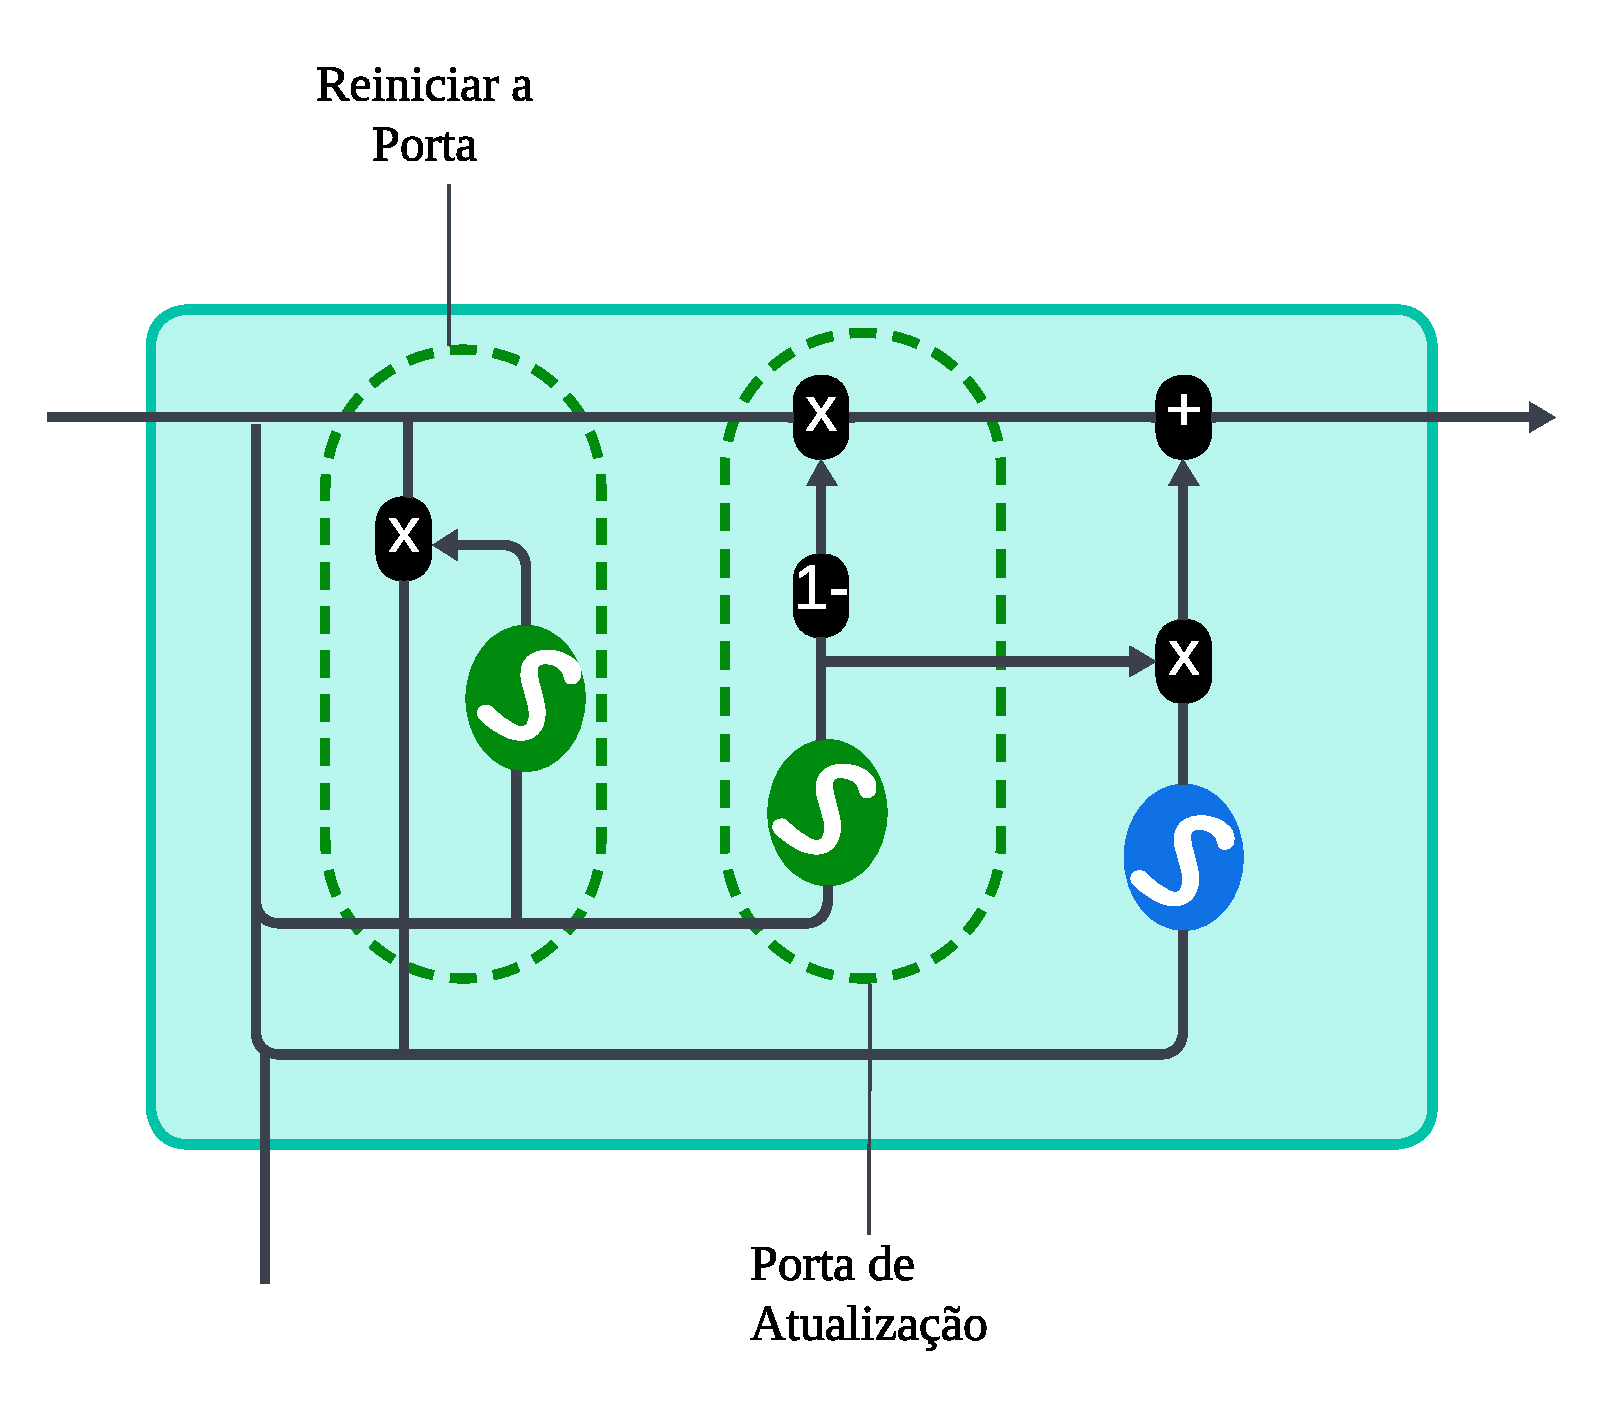
\includegraphics[width=0.5\linewidth]{Modelos/Figuras/gru.pdf}
\end{figure}
 
 As redes neurais GRUs, LSTMs, e RNNs apresentam variações em suas arquiteturas, todas projetadas para abordar a dificuldade de capturar dependências temporais em sequências de dados. Enquanto as RNNs tradicionais têm uma tendência a sofrer com o desvanecimento do gradiente ao longo do tempo, as LSTMs e GRUs foram desenvolvidas para superar essa limitação. As LSTMs introduzem células de memória e portas de controle que permitem armazenar e atualizar informações relevantes ao longo das etapas temporais, sendo especialmente adequadas para capturar relações de dependência de longo prazo. As GRUs, por sua vez, simplificam a arquitetura das LSTMs, utilizando portas de atualização para permitir o fluxo de informações e controle sobre o estado oculto.
 A Figura \ref{fig:rnn-vs-lstm-vs-gru-1024x308} ilustra as RNNs, LSTMs, e GRUs, permitindo uma visualização das diferenças entre essas redes neurais. Cada seção possui um diagrama da arquitetura da rede, com nós representando neurônios e arestas representando conexões entre neurônios. A RNN tem um único neurônio recorrente, a LSTM tem vários neurônios recorrentes com conexões adicionais que formam portões e células de memória, e a GRU tem dois portões que controlam o fluxo de informação na memória oculta da rede. 
 
 \begin{figure}[!htb]
 	\centering
 	\caption{Diferenças entre RNN, LSTM, e GRU.}
 	\label{fig:rnn-vs-lstm-vs-gru-1024x308}
 	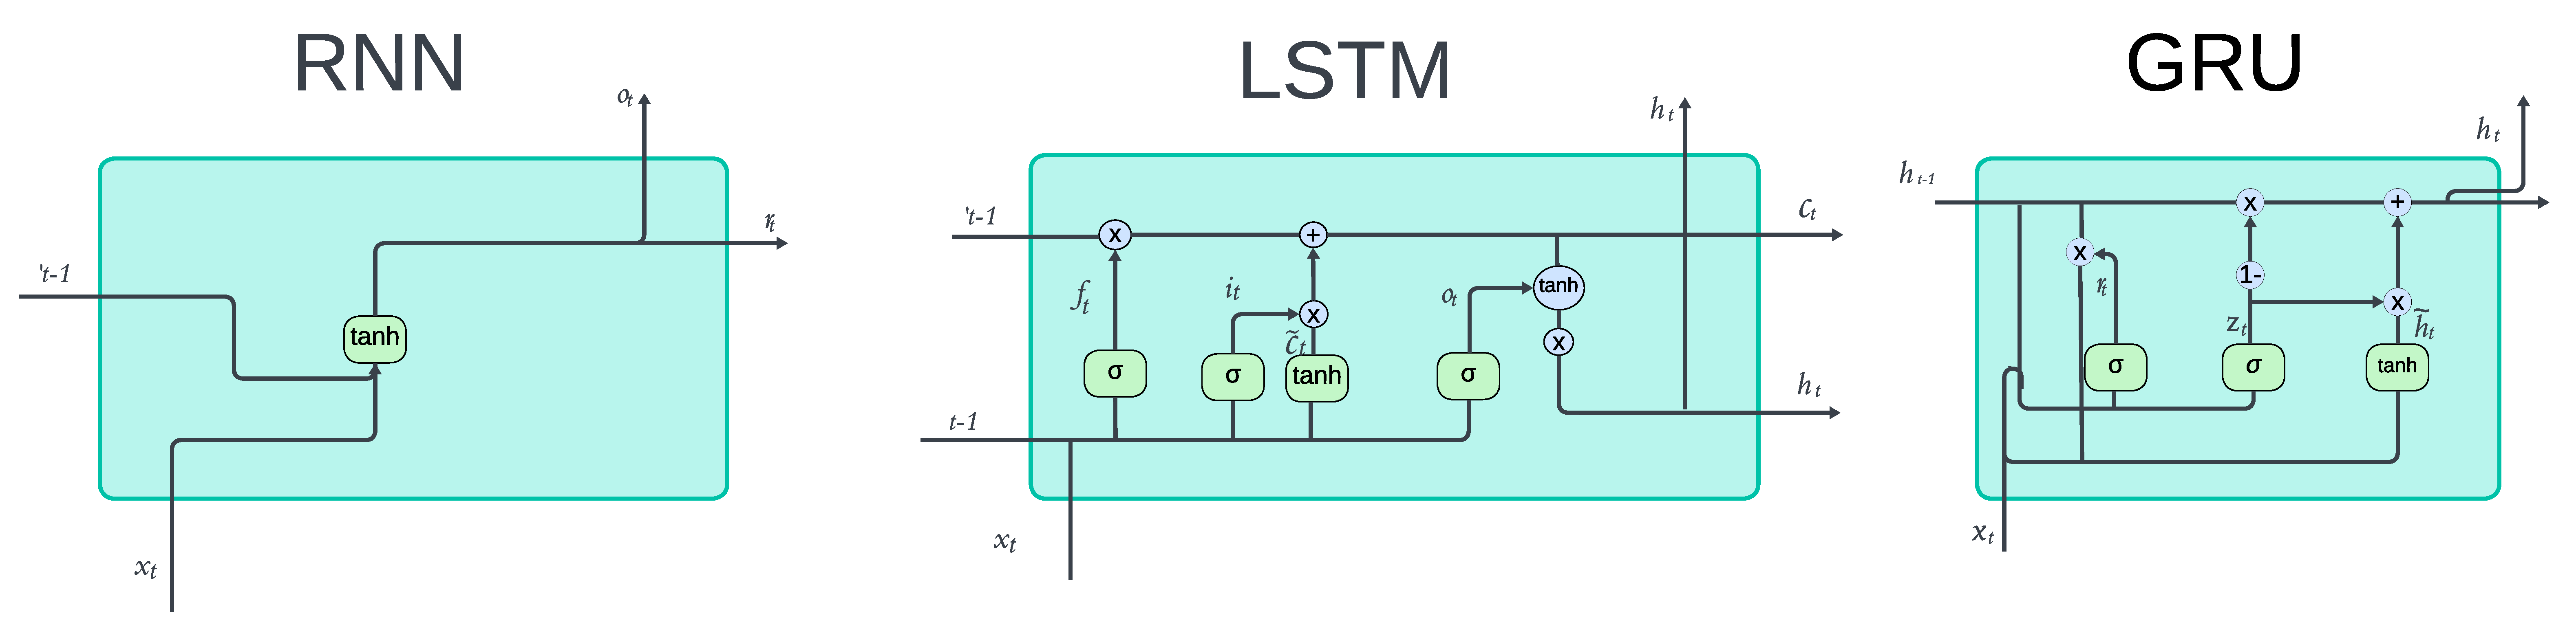
\includegraphics[width=\linewidth]{Modelos/Figuras/RNN-vs-LSTM-vs-GRU-1024x308.pdf}
 \end{figure}
 
  As LSTMs e GRUs oferecem soluções mais sofisticadas em relação às RNNs tradicionais, apresentando mecanismos que permitem capturar dependências de longo prazo de maneira mais eficaz.
 
 \subsection{Rede Neural Convolucional}
 
As Redes Neurais Convolucionais CNN são um tipo de rede neural que utiliza a operação de convolução em vez da multiplicação por matrizes em ao menos uma de suas camadas. Esse tipo de rede é efetiva em aplicações em que os dados são dispostos de forma que a relação de vizinhança entre os elementos é relevante, no caso de séries temporais, que são sequências unidimensionais de dados amostrados em intervalos de tempo regulares tem-se este tipo de característica \cite{silva_2021}, \cite{7533055} .
 
A camada convolucional tem como objetivo extrair as características mais importantes da entrada. Dessa forma, sua saída é um mapa de características obtido a partir da convolução da entrada com um \textit{kernel} aprendido, seguido da aplicação de uma função de ativação não linear \cite{lucas_2019}. Os mapas de características completos são obtidos por,
 
 \begin{eqnarray}
 	Z_{i, j, k}^L&=&W_k^L \cdot X_{i, j}^L+b_k^L\label{cnn}
 \end{eqnarray}
 
\noindent onde $Z_{i, j, k}^L$ é o mapa de características obtido pela convolução do k-ésimo filtro da \textit{L-ésima} camada com a célula de entrada centrada na localização $(i, j)$, $W_k^L$ vetor de pesos do \textit{k-ésimo} filtro da \textit{L-ésima} camada, $b_k^L$ termo de polarização do k-ésimo filtro da L-ésima camada,  $X_{i, j}^L$ é a célula de entrada centrada na localização $(i,j)$ da $L-$ésima camada.

A profundidade dos mapas de características é dada pelo número de \textit{kernels} (ou filtros) de convolução. Observe na Figura \ref{fig:cnn} que a $1^{\mathrm{a}}$
camada de convolução com 6 \textit{kernels} gera uma saída de profundidade 6. Isso porque, cada \textit{kernel} possui pesos diferentes para extrair diferentes características da entrada \cite{lucas_2019}.
 
 \begin{figure}[!htb]
 	\centering
 	\caption{Modelo de uma Rede Neural Convolucional.}
 	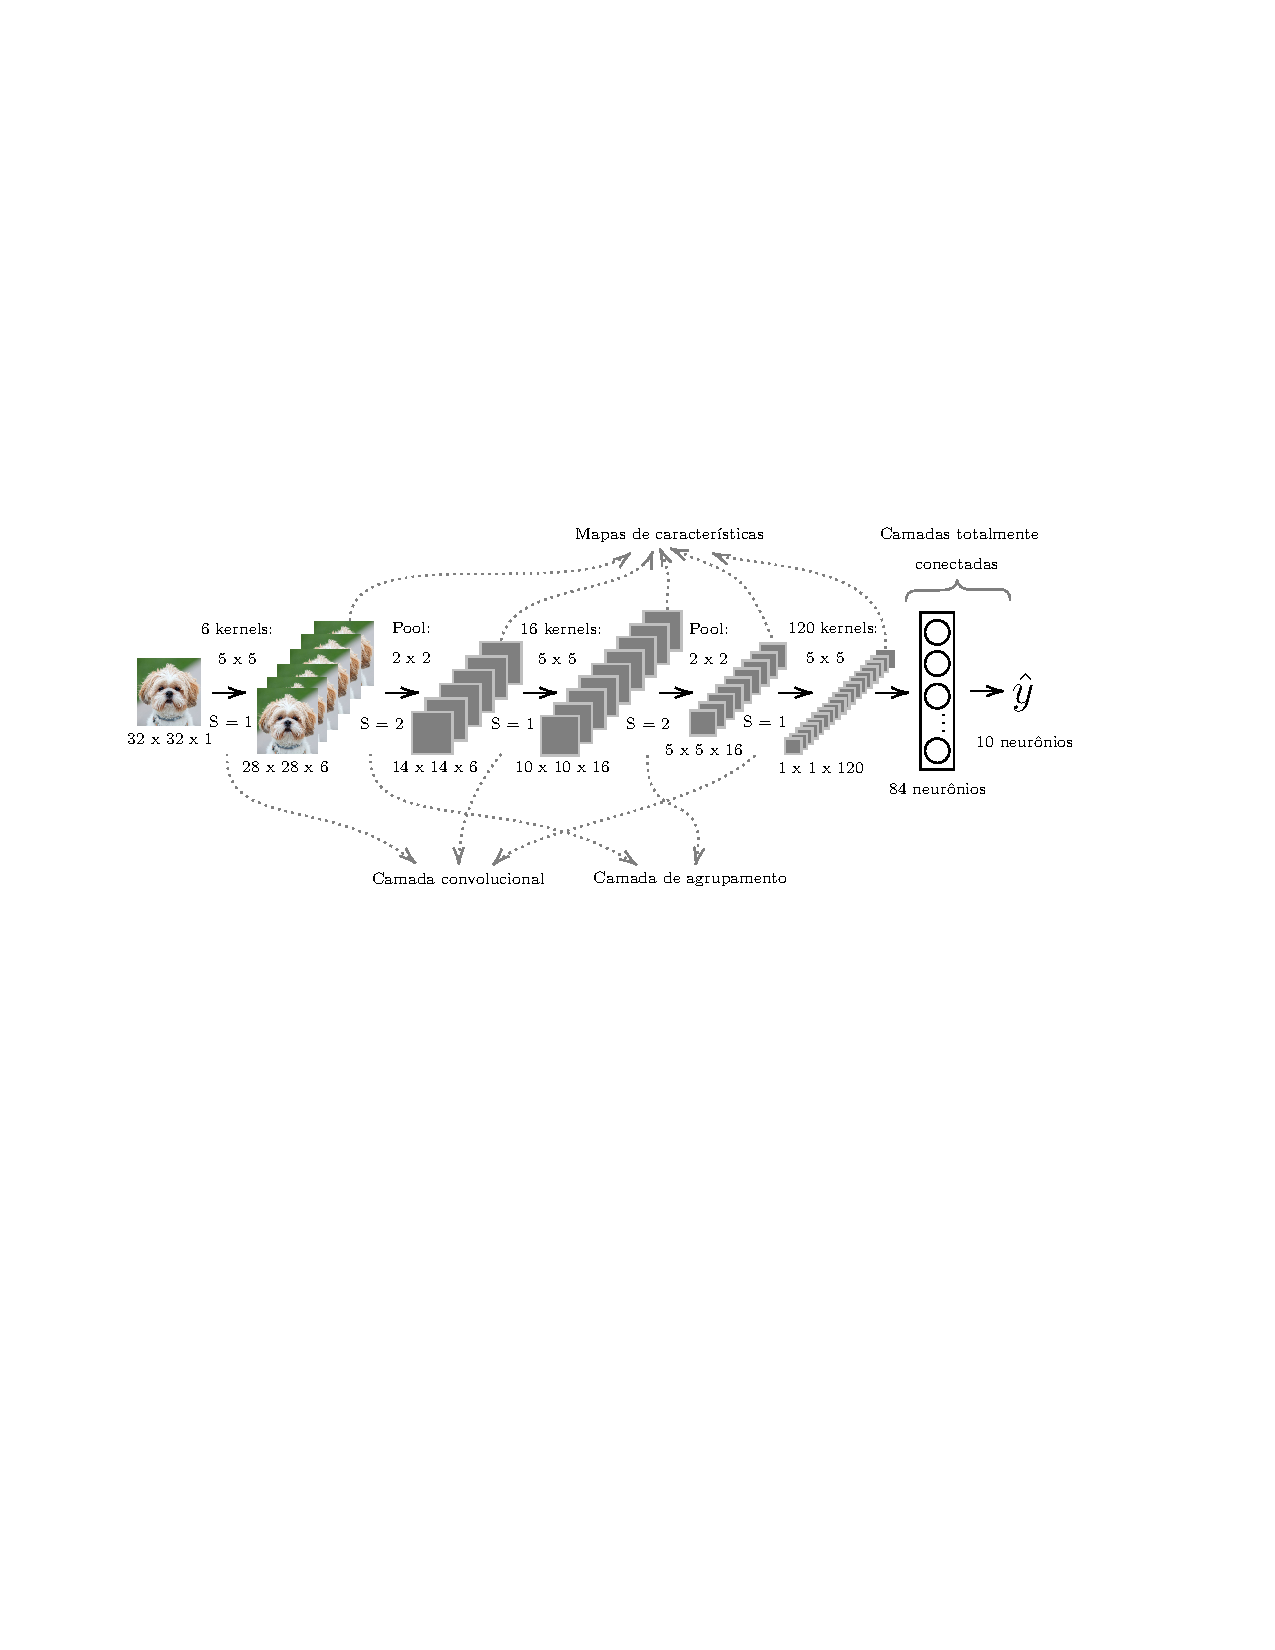
\includegraphics[width=1\linewidth]{Modelos/Figuras/cnn.pdf}
 	\label{fig:cnn}
 \end{figure}
  
Uma vantagem das camadas de convolução é o compartilhamento do vetor de pesos para toda a circunvolução na construção de um mapa de características, pois reduz o número de parâmetros na rede, resultando em treinamento e previsões mais eficientes \cite{lucas_2019}.
A largura e a altura desses mapas são definidas pelo tamanho do \textit{kernel} e do \textit{stride} (passo da circunvolução) dado por,
 
 \begin{eqnarray}
 	T_{\text {map }}&=&\left(\dfrac{I-F}{S+1}\right)\label{cnn1}
 \end{eqnarray}
 
 \noindent onde
 $T_{\text {map }}$ é a altura ou largura do mapa de características,
 $I$ é a altura ou largura da entrada,
 $F$ é a altura ou largura do \textit{kernel} de convolução,
 $S$ é o tamanho do \textit{stride}.
 
 \subsection{Medidas de Desempenho}\label{subsec:metrica}
 
As métricas estatísticas são utilizadas na análise de previsão de séries temporais para avaliar se o modelo preditor possui um desempenho adequado e/ou superior. Quanto menor for o erro da maioria das métricas, melhor será o desempenho do modelo aplicado.
 
A Raiz do Erro Médio Quadrático Relativo (RRMSE) é uma variante do erro quadrático médio (RMSE) sendo calculado por,
 
 \begin{eqnarray}
 	R R M S E&=&\dfrac{\sqrt{\frac{1}{n} \sum_{i=1}^n\left(y_i-\hat{y}_i\right)^2}}{\sum_{i=1}^n\left(\hat{y}_i\right)^2}
 \end{eqnarray}
 
 \noindent onde $n$ número total de observações ou amostras no conjunto de dados,
 $y_i$ valor real da observação $i$,
 $\hat{y}_i$ valor previsto ou estimado da observação $i$ pelo modelo,
 $\sum_{i=1}^{n}$ soma sobre todas as observações no conjunto de dados.
 
O Erro Absoluto Médio (MAE) é utilizado como uma métrica para avaliar o desempenho de modelos de previsão. Em vez de calcular a média das diferenças entre os valores reais e previstos, o MAE calcula a média dos valores absolutos dessas diferenças, garantindo que os erros positivos e negativos não se anulem, calculada por,
 
 \begin{eqnarray}
 	M A E &=& \dfrac{1}{n} \sum\left|y_i-\hat{y}_i\right|\label{eq:mae}
 \end{eqnarray}
 
 \noindent sua interpretação é similar ao RRMSE, em que o erro é expresso na mesma escala ou ordem de grandeza da variável estudada.
 
O Erro Percentual Absoluto Médio Simétrico (sMAPE) é outra métrica comumente utilizada para avaliar a precisão de modelos de previsão. O sMAPE é expresso como uma porcentagem, facilitando a compreensão da precisão relativa do modelo. O sMAPE é adequado para trabalhar com valores nulos nos dados, pois a divisão por zero é evitada no cálculo da métrica. O sMAPE é sensível a valores extremos nos dados. Se houver valores discrepantes que não representem a tendência geral, eles podem influenciar significativamente a métrica. Seu cálculo é dado por,
  
 \begin{eqnarray}
 	sMAPE &=& \dfrac{1}{n} \sum_{i=1}^{n} \dfrac{2|y_i - \hat{y}_i|}{(|y_i| + |\hat{y}_i|)} \times 100\label{eq:smape}
 \end{eqnarray}
 

\subsection{Correla\c c\~ao de Pearson}

A correlação de Pearson é uma medida estatística que avalia a relação linear entre duas variáveis. No contexto de séries temporais, a correlação de Pearson pode ser útil para entender se existe uma relação linear entre duas séries temporais, ou entre diferentes variáveis de uma mesma sérite temporal \cite{CESARDELIMANOGUEIRA2023128066}. No entanto, é importante ter em mente algumas considerações ao aplicar a correlação de Pearson a séries temporais: ($i$) a correlação de Pearson é sensível a tendências e sazonalidades nas séries temporais. Se houver uma tendência ou sazonalidade em ambas as séries, a correlação pode indicar uma relação mesmo que a relação real seja mais complexa. ($ii$) a correlação de Pearson pressupõe uma relação linear entre as variáveis. Se a relação entre as séries temporais for não linear, a correlação de Pearson pode não capturar essa relação de maneira adequada, e ($iii$) a correlação de Pearson pode ser sensível a valores extremos (\textit{outliers}) \cite{DOSSANTOSCOELHO2024129366}. Valores extremos podem distorcer a medida de correlação, tornando-a menos representativa da relação geral entre as séries.

Ao usar a correlação de Pearson para análise de séries temporais, é importante interpretar os resultados com cautela e considerar outros métodos estatísticos e gráficos para uma compreensão mais completa da relação entre as séries. A equação do coeficiente de correlação de Pearson é dada por:
 
 \begin{equation}
 	r=\frac{\sum\left(x_i-\bar{x}\right)\left(y_i-\bar{y}\right)}{\sqrt{\left(\sum\left(x_i-\bar{x}\right)^2\right)\left(\sum\left(y_i-\bar{y}\right)^2\right)}}
 \end{equation}
 
 \noindent onde $x_i$ e $y_i$ representam os valores das variáveis $X$ e $Y$, respectivamente. $\bar{x}$ e $\bar{y}$ são as médias dos valores $x_i$ e $y_i$. 
 
O coeficiente de correlação de Pearson mede a força e a direção da relação linear entre as variáveis $X$ e $Y$. Valores próximos a 1 indicam uma correlação positiva forte, valores próximos a $-1$ indicam uma correlação negativa forte, e valores próximos a $0$ indicam  ausência de correlação entre as variáveis.
 
\subsection{Decomposi\c c\~ao STL}
 
A decomposição STL é uma técnica amplamente utilizada para decompor séries temporais em seus componentes sazonais, de tendência e restantes \cite{RIBEIRO2023112982}. O método STL realiza a decomposição aditiva dos dados por meio de uma sequência de aplicações do Loess mais suave, onde regressões polinomiais ponderadas localmente são aplicadas em cada amostra do conjunto de dados, tendo como variáveis explicativas os valores próximos do amostra cuja resposta está sendo estimada \cite{Theodosiou20111178}.
 
Ao aplicar a decomposição STL, a série temporal pode ser expressa como a soma dos componentes sazonais, de tendência e restantes. Essa técnica se revela valiosa para análise e modelagem de séries temporais, fornecendo uma compreensão clara dos padrões de variação presentes nos dados. Este método prepara o terreno para uma abordagem mais refinada na aplicação de modelos, permitindo uma interpretação mais precisa e uma melhor adaptação aos padrões intrínsecos dos dados ao utilizar o ARIMA ou SARIMA em sua análise \cite{RIBEIRO2023112982}.
 
A decomposição STL é formalmente definida como:
 
 \begin{eqnarray}
 	y_t=f\left(S_t, T_t, R_t\right)&=&\left\{\begin{array}{l}
 		y_t=S_t+T_t+R_t \quad \text { modelo aditivo } \\
 		y_t=S_t T_t R_t \quad \text { modelo multiplicativo }
 	\end{array}\right. \label{eq:stl}
 \end{eqnarray}

\noindent onde $y_t$ é o valor da série temporal no tempo $t$, $T_t$ é a componente de tendência no tempo $t$, $S_t$ é a componente de sazonalidade no tempo $t$, $R_t$ é a componente de resíduo no tempo $t$.

\subsection{Teste Run}

O teste de Run, também conhecido como teste de sequências de \textit{Wald-Wolfowitz}, verifica se uma série de dados foi gerada aleatoriamente \cite{PAIVA}.

As hipóteses são:
$$
\left\{\begin{array}{l}
	H_0: \text { a sequência foi gerada aleatoriamente (sem tendência) } \\
	H_1: \text { a sequência não foi gerada aleatoriamente (possui uma tendência). }
\end{array}\right.
$$

A estatística $T_1$ utiliza os valores acima e abaixo da mediana. Primeiramente, considera-se $N$ como o número de observações em uma série. Em seguida, esses valores são ordenados e o símbolo $A$ é atribuído quando o valor da observação é maior ou igual à mediana, $A \geq m$, e o símbolo $B$ se o valor for menor que a mediana, $B<m$.

O número total de observações é $N=\left(n_1\right.$ pontos $\left.\mathrm{A}\right)+\left(n_2\right.$ pontos B $)$, com a estatística $T_1$ igual ao número de sequências ou número de execuções.

O valor de $T_1$ é obtido contando o número de sequências iguais, ou seja, o número de oscilações no conjunto de dados entre os valores $A$ e $B$. Por exemplo, suponha que o número de observações seja igual a 20. Entre essas observações, os primeiros 5 valores eram iguais a $A$, os próximos 6 eram iguais a $B$ e os outros valores eram iguais a $A$ novamente. Então, 3 sequências $(A B A)$ foram obtidas, ou seja, o número de sequências (ou execuções) é igual a 3.

Conforme \citeonline{PAIVA}, no caso de poucas sequências em relação à série, a hipótese nula $H_0$ é rejeitada. Para valores de $n_1$ ou $n_2>20$, a distribuição normal é utilizada sob $H_0$, ou seja, $T_1 \sim N\left(\mu, \sigma^2\right)$, onde

\begin{eqnarray}
	\mu&=&\dfrac{2 n_1 n_2}{N}+1, \\
	\nonumber\\
	 \sigma&=&\sqrt{\dfrac{2 n_1 n_2\left(2 n_1 n_2-N\right)}{N^2(N-1)}} 
\end{eqnarray}


Através dos cálculos de $\mu$ e $\sigma$, pode-se encontrar o valor da estatística $\mathrm{Z}$ dada por:

\begin{eqnarray}
	Z&=&\frac{T_1-\mu}{\sigma}
\end{eqnarray}


Analisando o valor de $Z$, $H_0$ é rejeitada se $|Z|>Z_{\frac{a}{2}}$, sendo $\alpha$ o nível de significância adotado.



\subsection{Teste Dickey-Fuller}

O teste Dickey-Fuller (DF) segue uma regressão linear AR de primeira ordem e testa a hipótese nula de que uma raiz unitária está presente em uma série temporal, indicando a não estacionariedade. A forma mais comum do teste Dickey-Fuller é conhecida como \textit{Augmented Dickey-Fuller} (ADF) , que inclui termos adicionais na regressão para trabalhar com possíveis problemas de autocorrelação
 \cite{Agiakloglou}. O procedimento geral do teste DF envolve as seguintes etapas:

Formulação da Hipótese Nula ($H_0$): A hipótese nula assume a presença de raízes unitárias, o que indica não estacionariedade na série temporal.
Formulação da Hipótese Alternativa ($H_1$): A hipótese alternativa busca rejeitar a hipótese nula, sugerindo a estacionariedade da série temporal.
Realização do Teste: O teste DF é realizado calculando uma estatística de teste. Se o valor de p associado à estatística de teste for menor que um determinado nível de significância pré-definido, a hipótese nula é rejeitada.
Interpretação dos Resultados: Se a hipótese nula for rejeitada, isso sugere que a série temporal é estacionária. Caso contrário, a não estacionariedade da série temporal não pode ser descartada.

De acordo com o \citeonline{Reisen2017115}, o teste DF é representado por,



\begin{eqnarray}
	 \Delta y(t)&=&\alpha+\beta \cdot t+\gamma \cdot y(t-1)+\delta_1 \cdot \Delta y(t-1)+\delta_2 \cdot \Delta y(t-2)+\ldots+\delta_p \nonumber\\ 
	&&\Delta y(t-p)+\varepsilon(t)
\end{eqnarray}

\noindent onde $\Delta y(t)$ é a diferença entre os valores consecutivos da série temporal no tempo $t$, $y(t-1)$ é o valor da série temporal no tempo anterior, $t$ é uma variável de tendência temporal, $\alpha, \beta, \gamma$ são parâmetros a serem estimados, $\delta_1, \delta_2, \ldots, \delta_p$ são os coeficientes associados às diferenças defasadas, $\varepsilon(t)$ é o termo de erro.
 
 \subsection{Teste de Ljung-Box}
 
A ideia do teste de Ljung-Box é verificar se as autocorrelações dos resíduos em diferentes defasagens são estatisticamente diferentes de zero. Se a estatística de teste do Ljung-Box indicar significância estatística, isso sugere que há autocorrelações remanescentes nos resíduos, indicando que o modelo não está capturando completamente a estrutura da série temporal \cite{box}, \cite{ljung}, \cite{dav}. As etapas básicas do teste de Ljung-Box:

Formulação da Hipótese Nula ($H_0$): A hipótese nula assume que não há autocorrelação nos resíduos.
Formulação da Hipótese Alternativa ($H_1$): A hipótese alternativa sugere que há autocorrelação nos resíduos.
Cálculo da Estatística de Teste: A estatística de teste de Ljung-Box é calculada usando as autocorrelações dos resíduos em várias defasagens. A fórmula é baseada na soma dos quadrados dessas autocorrelações.
Distribuição da Estatística de Teste: A estatística de teste é comparada a uma distribuição qui-quadrado com um número apropriado de graus de liberdade. Isso depende do número de defasagens considerado no teste.
Decisão Estatística: Se o valor de p associado à estatística de teste for menor que um nível de significância escolhido (por exemplo, $0,05$), a hipótese nula é rejeitada, indicando a presença de autocorrelação nos resíduos.
 
A estatística de teste Box-Pierce é uma versão simplificada da estatística de Ljung-Box para a qual estudos de simulação subsequentes mostraram baixo desempenho \cite{dav}. A estatística de teste é \cite{ljung}:
 
 \begin{eqnarray}
 	Q&=&n(n+2) \sum_{k=1}^h \dfrac{\hat{\rho}_k^2}{n-k}
 \end{eqnarray}
 
\noindent onde $n$ é o tamanho da amostra, $\hat{\rho}_k$ é a autocorrelação da amostra no lag $k$ e $h$ é o número de defasagens que estão sendo testadas. Debaixo $H_0$ a estatística $Q$ segue assintoticamente um $\chi_{(h)}^2$. Para o nível de significância $\alpha$, a região crítica para rejeição da hipótese de aleatoriedade é:
 
\begin{eqnarray}
 	Q&>&\chi_{1-\alpha, h}^2
\end{eqnarray}
 
\noindent onde $\chi_{1-\alpha, h}^2$ é o $(1-\alpha)-$ quantil \cite{Brockwell2002} da distribuição qui-quadrada com graus $h$ de liberdade.
 
O teste de Ljung-Box é comumente usado na modelagem de média móvel integrada ARIMA. Note que ele é aplicado aos resíduos de um modelo ARIMA ajustado, não à série original, e em tais aplicações a hipótese que está sendo testada é que os resíduos do modelo ARIMA não têm autocorrelação. Ao testar os resíduos de um modelo ARIMA estimado, os graus de liberdade precisam ser ajustados para refletir a estimação do parâmetro. Por exemplo, para um modelo ARIMA $(p,0,q)$, os graus de liberdade devem ser definidos como $h-p-q$ \cite{Davidson2000}. O teste Box-Pierce utiliza a estatística do teste, na notação descrita previamente, dada por \cite{box}
 
 \begin{eqnarray}
 	Q_{\mathrm{BP}}=n \sum_{k=1}^h \hat{\rho}_k^2
 \end{eqnarray}
 
\noindent e usa a mesma região crítica definida previamente.
Estudos de simulação mostraram que a distribuição para a estatística Ljung-Box é mais próxima de um $\chi^2_{(h)}$ $6$ distribuição do que é a distribuição para a estatística Box-Pierce para todos os tamanhos de amostra, incluindo os pequenos.
 
 
\subsection{Testes de Hip\'oteses}
 
O teste de Friedman classifica os modelos $K$ em cada conjunto de dados em relação ao valor absoluto dos resultados dados por esses algoritmos. A classificação do algoritmo com maior desempenho é $1$ , e o com menor desempenho é classificado como $\mathrm{K}$. Em seguida, o valor da estatística com base em todas as classificações é calculado como mostrado em equações \eqref{ff} e \eqref{fx} com $r_{e u}^j$ sendo a classificação do desempenho do $j$-ésimo algoritmo no $i$-ésimo conjunto de dados. Essa estatística obedece à distribuição do qui-quadrado com $\mathrm{K}-1$ graus de liberdade \cite{Liu2022}.
 
 \begin{eqnarray}
 	\chi_F^2 & =&\frac{12 N}{K(K+1)}\left[\sum_{j=1}^K R_j^2-\frac{K(K+1)^2}{4}\right] \label{ff}\\
 	R_j & =&\frac{1}{N} \sum_{i=1}^N r_{e i l}^j \label{fx}\\
 	F_F&=&\dfrac{(N-1) \chi_F^2}{N(K-1) \chi_F^2}\label{fx1}
 \end{eqnarray}
 
 
As estatísticas $F_F$ mostrados na equação \eqref{fx1} obedecem à distribuição F com graus de liberdade $K-1$ e $(K-1)$ $(N-1)$. Pode-se obter o valor crítico abaixo do nível de significância especificado (geralmente $\alpha = 0,05$ ou $0,01$). Ao comparar esse valor crítico com o valor calculado com a equação \eqref{fx1}, a hipótese nula é rejeitada se o valor estatístico $F_F$ é maior que o valor crítico, indicando que há diferenças significativas entre os algoritmos $K$. Em seguida, pode-se realizar um procedimento \textit{post hoc} para analisar se o desempenho do algoritmo de controle é significativamente superior ao de cada algoritmo de referência nos experimentos. Ao contrário, se o valor for menor ou igual ao valor crítico, a hipótese nula é aceita, indicando que não há diferenças significativas entre os algoritmos $K$.
  
Adicionalmente, foi empregada a \textit{Critical Difference} (CD) para avaliar se dois regressores eram significativamente distintos entre si. O CD foi calculado de acordo com a fórmula mencionada anteriormente:

\begin{equation}
	CD = q_\alpha \sqrt{\frac{K(K+1)}{6N}}
\end{equation}

\noindent Na equação do CD, $q_\alpha$ representa o valor crítico obtido das Tabelas \ref{tb:nemenyi} e \ref{tb:nemeyirede} de teste de Nemenyi, $k$ é o número de regressores, e $N$ é o número total de amostras \cite{Liu2022}.
 
 
 \subsection{Otimiza\c c\~ao}
 
A utilização do \textit{Tree-structured Parzen Estimator} (TPE) na otimização de hiperparâmetros é crucial para melhorar o desempenho dos modelos. Integrado à biblioteca Optuna, ele desempenha um papel vital ao guiar a busca eficiente por conjuntos ideais de hiperparâmetros durante a otimização automática \cite{tpe}.

Ao dividir o espaço de busca, o TPE destaca-se ao identificar áreas promissoras para exploração, direcionando a análise de maneira inteligente e eficiente. Essa capacidade de focar em regiões promissoras contribui significativamente para a melhoria do desempenho do modelo.

No contexto da demanda de água, a otimização de modelos é essencial para prever e gerenciar eficientemente o consumo de água. A correlação aqui reside na importância de ajustar os hiperparâmetros do modelo para otimizar sua precisão na previsão da demanda de água. O TPE, ao guiar a busca por configurações ideais, contribui para modelos mais precisos e adaptáveis \cite{tpe}.

A equação fundamental do TPE, ao maximizar a probabilidade de melhoria, reflete o compromisso em encontrar conjuntos ótimos de hiperparâmetros. Essa abordagem probabilística, aplicada à otimização, permite ajustes dinâmicos ao longo do tempo, garantindo que o modelo se adapte às mudanças nas demandas da previsão de água.

$$ P(x \mid y) = \begin{cases} 
	p(x), & \text{se } y > y^* \\
	q(x), & \text{se } y \leq y^*
\end{cases} $$

\noindent onde $ x $ representa um conjunto de hiperparâmetros, $ y $ é o valor da função objetivo associado a esses hiperparâmetros, $ y^* $ é o valor de referência para a melhoria, $ p(x) $ é a probabilidade de $ x $ ser um conjunto bom de hiperparâmetros, $ q(x) $ é a probabilidade de $ x $ ser um conjunto ruim de hiperparâmetros.

Assim, ao considerar a otimização de hiperparâmetros com o TPE, não apenas aprimoramos a eficiência dos modelos, mas também fortalecemos sua capacidade de contribuir para soluções mais precisas e adaptáveis em domínios cruciais, como o gerenciamento da demanda de água.
